\documentclass[]{article}
\PassOptionsToPackage{numbers,compress}{natbib}
\usepackage{jmlr2e}
\usepackage{url}
\usepackage{amsmath}
\usepackage{amssymb}
\usepackage{amsbsy}
\usepackage{siunitx}
\usepackage{algorithm}
\usepackage{algorithmicx}
\usepackage{algpseudocode}
\usepackage{mathtools}
\usepackage{array}
\usepackage{setspace}
%\usepackage{caption}
\usepackage{subcaption}
\usepackage{booktabs}
\usepackage{adjustbox}
\usepackage{microtype}

\usepackage{times}
\usepackage{footmisc}
\usepackage{listings}
\usepackage{color}
\usepackage{xcolor}
\usepackage{textcomp}
\usepackage{xspace}

\usepackage{fancyhdr}


\usepackage{bibentry}
\nobibliography*

\usepackage{paralist}

\usepackage{natbib}
%\bibliographystyle{abbrvnat-simple}
%\setlength{\bibsep}{2.0pt}
%
%\setlength{\floatsep}{5pt plus 2pt minus 2pt}
%\setlength{\textfloatsep}{5pt plus 2pt minus 2pt}
%\setlength{\intextsep}{5pt plus 2pt minus 2pt}

\usepackage{enumitem}
\setlist[itemize]{leftmargin=*}

\usepackage{hyperref}

%\graphicspath{{./figures/}}

\definecolor{darkgreen}{rgb}{0.25,.5,0}
\definecolor{blue}{rgb}{0,0.33,0.66}
\definecolor{red}{rgb}{0.66,0.0,0.0}
\definecolor{purple}{rgb}{0.33,0,0.66}
\definecolor{cyan}{rgb}{0.0,0.5,0.5}
\definecolor{orange}{rgb}{0.5,0.25,0.0}
\definecolor{gray}{rgb}{0.4,0.4,0.4}
\lstset{ 
	language=Lisp, 
	basicstyle=\small\ttfamily,
	keywordstyle={}, 
	alsoletter={/},
	alsoletter={:},
	alsoletter={*},
	alsoletter={<-},
	commentstyle=\em \color{gray}, 
	frame=lines,
	%float=tbph,
	% captionpos=b,
	showstringspaces=false, 
	keywordstyle=[1]\bf\ttfamily\color{blue},
	keywords=[1]{BO,theta-best,bo-acquire,sample-initial-points,sample,observe,observe*,observe<-,predict,store,retrieve,return,catch,throw},
	keywordstyle=[2]\bf\ttfamily\color{red},
	keywords=[2]{defn,if,let,letfn,loop,looppredict,recur},
	keywordstyle=[3]\bf\ttfamily\color{cyan},
	keywords=[3]{absorb,assoc,argmax,count,cons,conj,dirichlet-discrete,do,exponential,first,flip,fn,gamma,beta,get,keys,lazy-seq,map,mvn-niw,nth,mat/add,mat/div,normal,print,produce,reduce,repeat,repeatedly,rest,set,shape,take,uniform-continuous,vec,distribution,factor,simulate,abc-likelihood,when,max},
	keywordstyle=[4]\bf\ttfamily\color{purple},
	keywords=[4]{defopt,defquery,doopt,doquery,query,defdist},
	keywordstyle=[5]\ttfamily\color{orange},
	keywords=[5]{:nu,:alpha,:id},
	mathescape=true,
	stringstyle={},
} 
\lstnewenvironment{code}[2]{\lstset{caption=#1,label=#2}}{}

\newcommand{\lsi}[1]{\lstinline$#1$}

\newcommand{\sample}{\lstinline$sample$\xspace}
\newcommand{\observe}{\lstinline$observe$\xspace}
\newcommand{\observes}{\lstinline$observe<-$\xspace}
\newcommand{\predict}{\lstinline$predict$\xspace}
\newcommand{\simulatec}{\lstinline$simulate$\xspace}
\newcommand{\abcl}{\lstinline$abc-likelihood$\xspace}
\newcommand{\factor}{\lstinline$factor$\xspace}

\newcommand{\defdist}{\lstinline$defdist$\xspace}
\newcommand{\defquery}{\lstinline$defquery$\xspace}
\newcommand{\query}{\lstinline$query$\xspace}
\newcommand{\defopt}{\lstinline$defopt$\xspace}
\newcommand{\doquery}{\lstinline$doquery$\xspace}
\newcommand{\doopt}{\lstinline$doopt$\xspace}
\newcommand{\normal}{\lstinline$normal$\xspace}
\newcommand{\betaa}{\lstinline$beta$\xspace}
\newcommand{\gammaa}{\lstinline$gamma$\xspace}

%\newcommand{\observe}{\texttt{\small\bf\color{darkgreen} observe}\xspace}
%\newcommand{\predict}{\texttt{\small\bf\color{darkgreen} predict}\xspace}
%\newcommand{\sample}{\texttt{\small\bf\color{darkgreen} sample}\xspace}
%\newcommand{\defquery}{\texttt{\small\bf\color{darkgreen} defquery}\xspace}
%\newcommand{\normal}{\texttt{\small\bf\color{blue} normal}\xspace}
%\newcommand{\boaq}{\texttt{\small\bf\color{blue} bo-acquire}\xspace}
%\newcommand{\sampleinitpoints}{\texttt{\small\bf\color{blue} sample-initial-points}\xspace}

%\newcommand{\defopt}{\texttt{\small\bf\color{darkgreen} defopt}\xspace}
%\newcommand{\doopt}{\texttt{\small\bf\color{darkgreen} doopt}\xspace}
%\newcommand{\doquery}{\texttt{\small\bf\color{darkgreen} doquery}\xspace}
%\newcommand{\defdist}{\texttt{\small\bf\color{darkgreen} defdist}\xspace}

%\usepackage{wrapfig,lipsum,booktabs}

%\usepackage{hyperref}


\newcolumntype{A}{>{\centering\arraybackslash}m{1cm}}

\newcolumntype{B}{>{\centering\arraybackslash}m{1.5cm}}

\newcolumntype{D}{>{\centering\arraybackslash}m{2cm}}

\renewcommand*\Call[2]{\textproc{#1}(#2)}

\algnewcommand{\IIf}[1]{\unskip \algorithmicif\ #1\ \algorithmicthen}
\algnewcommand{\ElseIIf}{\unskip\ \algorithmicelse}
\algnewcommand{\EndIIf}{\unskip\ \algorithmicend\ \algorithmicif}

\newcommand{\mX}{\mathcal{X}}
\newcommand{\mD}{\mathcal{D}}
\newcommand{\nx}{_{\mathrm{next}}}
\newcommand{\real}{\mathbb{R}}
\newcommand{\xpos}{\tilde{\mathbf{x}}}
\newcommand{\xb}{\mathbf{x}}
\newcommand{\yb}{\mathbf{y}}
\newcommand{\zb}{\mathbf{z}}
\newcommand{\hb}{\mathbf{h}}
\newcommand{\hx}{h\left(\xb,\zb\right)}

\newcommand{\hu}{\hat{u}}
\newcommand{\hz}{\hat{Z}}
\newcommand{\hw}{\hat{w}}
\newcommand{\hth}{\hat{\theta}}
\newcommand{\ho}{\hat{\Omega}}

\newcommand{\tilz}{\tilde{Z}}
\newcommand{\tilw}{\tilde{w}}
\newcommand{\tilth}{\tilde{\theta}}
\newcommand{\tilo}{\tilde{\Omega}}

\newcommand{\jsm}{j^*_m}

\newcommand{\bc}{\left(\cdot\right)}
\newcommand{\bcc}{\left(\cdot\right)}
\newcommand{\mM}{\mathcal{M}}
\newcommand{\tx}{\texttt{x}}
\newcommand{\ty}{\texttt{y}}
\newcommand{\tz}{\texttt{z}}
\newcommand{\tb}{\texttt{b}}
\newcommand{\ft}{f\left(\theta\right)}
\newcommand{\tth}{\tilde{\theta}}
\newcommand{\mut}{\mu_m\left(\theta ; \alpha\right)}
\newcommand{\kt}{k_{m}\left(\theta,\theta'\right)}
\newcommand{\sut}{\sigma_m\left(\theta ; \alpha\right)}
\newcommand{\gut}{\gamma_{m}\left(\theta\right)}

\newcommand{\RN}[1]{%
	\textup{\uppercase\expandafter{\romannumeral#1}}%
}
\renewcommand{\v}[1]{\ensuremath{\boldsymbol{#1}}}

\DeclareMathOperator*{\argmax}{arg\,\!max}
\DeclareMathOperator{\Normal}{Normal}
\DeclareMathOperator{\Dirichlet}{Dirichlet}
\DeclareMathOperator{\Gammaa}{Gamma}
\DeclareMathOperator{\simulate}{simulate}
\DeclareMathOperator{\dist}{dist}
\DeclareMathOperator{\std}{std}


\newcommand{\qmarg}{\texttt{q-marg}}
\newcommand{\qprior}{\texttt{q-prior}}
\newcommand{\qacq}{\texttt{q-acq}}


\ShortHeadings{Bayesian Optimization for Probabilistic Programs}{Rainforth, Le, van de Meent, Osborne and Wood}
\firstpageno{1}

\title{Bayesian Optimization for Probabilistic Programs$^*$}

\author{\name Tom Rainforth \email twgr@robots.ox.ac.uk \\
	\addr Department of Engineering Science, University of Oxford
	\AND
	\name Tuan Anh Le \email tuananh@robots.ox.ac.uk \\
	\addr Department of Engineering Science, University of Oxford
	\AND
	\name Jan-Willem van de Meent \email j.vandemeent@northeastern.edu \\
	\addr College of Computer and Information Science, Northeastern University
	\AND
	\name Michael A Osborne \email mosb@robots.ox.ac.uk \\
	\addr Department of Engineering Science, University of Oxford
	\AND
	\name Frank Wood \email fwood@robots.ox.ac.uk \\
	\addr Department of Engineering Science, University of Oxford \\
}

\fancypagestyle{empty}{%
	\fancyhf{}% Clear header/footer
	\fancyhead[L]{}% Your journal/note
	\renewcommand{\headrulewidth}{0pt}
	\renewcommand{\footrulewidth}{0pt}
	\fancyfoot[L]{\footnotesize \vspace{-25pt} \rule{\textwidth}{0.4pt} \indent{} \indent{} *Please cite this version: \\ \vspace{5pt} \hspace{20pt} \begin{minipage}{0.9\textwidth}\bibentry{rainforth2016bayesian}\end{minipage}}% Your logo/image
}

\begin{document}
%
%\input{coverArXiv.tex}
%\newpage

\maketitle
\vspace{-30pt}

\newcommand\blfootnote[1]{%
	\begingroup
	\renewcommand\thefootnote{}\footnote{#1}%
	\addtocounter{footnote}{-1}%
	\endgroup
}

\begin{abstract}
% !TEX root = ../main.tex

\vspace{20pt}
Imagine a world where computational simulations can be inverted as easily as running them forwards, where data
can be used to refine models automatically, and where the only expertise one needs to carry
out powerful statistical analysis is a basic proficiency in scientific coding.  Creating such a
world is the ambitious long-term aim of \emph{probabilistic programming}.

The bottleneck for improving the probabilistic models, or simulators, used throughout the quantitative sciences,
is often not an ability to devise better models conceptually,  but a lack of expertise,
time, or resources to realize such innovations.
Probabilistic programming systems (PPSs) help alleviate this bottleneck 
by providing an expressive and accessible modeling framework,
%, often more in line we conventional scientific simulation than mainstream statistical approaches,
 then
automating the required computation to draw inferences from the model, for example finding
the model parameters likely to give rise to a certain output.
By decoupling model specification and inference, PPSs 
streamline the process of developing and drawing inferences from new models, while
opening up powerful statistical methods to non-experts.
%open up powerful statistical methods 
%to non-experts, while
%streamlining the process of developing new models or inference algorithms
%those within the machine learning and statistics communities.  
Many systems further provide
the flexibility to write new and exciting models which would be hard, or even impossible, to convey using 
conventional statistical frameworks.

The central goal of this thesis is to improve and extend PPSs.
%, providing some of the many steps
%that will be necessary to achieve the lofty long-term aims of the field.  
In particular, we will
make advancements to the underlying inference engines and increase the
range of problems which can be tackled.  For example, we will extend PPSs to a mixed inference-optimization
framework, thereby providing automation of tasks
such as model learning and engineering design.  Meanwhile, we make inroads into constructing systems
for automating adaptive sequential design problems, providing potential applications across the sciences.
Furthermore, the contributions of the work reach far beyond probabilistic programming, as 
achieving our goal will require us to make
advancements in a number of related fields such as particle Markov chain Monte Carlo methods,
Bayesian optimization, and Monte Carlo fundamentals. %, and Bayesian experimental design.

%
%Specifically, we will introduce \emph{interacting particle
%	Markov chain Monte Carlo},
%a new inference algorithm suitable for large-scale computation, and 
%detail is implementation as a general purpose inference engine for the PPS \emph{Anglican}. 
%%explain how it can be
%%used as general purpose inference engine for PPSs by detailing its implementation
%%in the PPS \emph{Anglican}.  
%We will extend PPSs beyond their typical inference setting
%to a more general mixed inference-optimization framework by introducing~\emph{Bayesian
%	optimization for probabilistic programs}, thereby providing automation of tasks
%such as model learning and engineering design.
%%in the same manner as inference is automated in existing systems.  
%We will develop theoretical 
%results on \emph{nesting Monte Carlo
%	estimators} and explain the important implications these have for nesting models in PPSs.
%Finally, we will 
%%examine a particular
%%class of nested estimation problems, those of Bayesian experimental design, and 
%introduce a high-level framework for automating adaptive sequential design problems, 
%%a particle example 
%providing application of our technique to psychological trials.
%%Finally, we will examine a particular
%%class of nested estimation problems, those of Bayesian experimental design, and introduce
%%a high-level framework for automating arbitrary adaptive sequential design problems,
%%providing application our technique to psychological trials.
%\blfootnote{\hspace{-20pt}*Please cite this version: \\ \bibentry{rainforth2016bayesian}}
\end{abstract}

\thispagestyle{empty}


\section{Introduction} 
\label{sec:IntroductionBOPP}

% !TEX root = ../main.tex

% Intro, contribution statement and related work
\subsection{Introduction}
\label{sec:ipmcmc:intro}
%In this paper we propose the interacting particle Markov chain Monte Carlo (\ipmcmc), a particle Markov chain Monte Carlo (\pmcmc) method that is suitable to execution on distributed and multi-core computing architectures and present empirical results suggesting significant improved mixing rates relative to both non-interacting \pg nodes and a single \pg node with an identical computational budget. 

%In this paper we present a Markov chain Monte Carlo (\mcmc) method that employs a pool of particle Markov chain Monte Carlo (\pmcmc) and sequential Monte Carlo (\smc) samplers. 


In this paper we propose the interacting particle Markov chain Monte Carlo (\ipmcmc) sampler. In \ipmcmc we run a pool of \csmc and unconditional \smc algorithms as parallel processes that we refer to as nodes. After each run of this pool, we apply successive Gibbs updates to the indexes of the \csmc nodes, such that the indices of the \csmc nodes changes. Hence, the nodes from which retained particles are sampled can change from one MCMC iteration to the next. This lets us trade off exploration (\smc) and exploitation (\csmc) to achieve improved mixing of the Markov chains. Crucially, the pool provides numerous candidate indices at each Gibbs update, giving a significantly higher probability that an entirely new retained particle will be ``switched in'' than in non-interacting alternatives.

This interaction requires only minimal communication; each node must report an estimate of the marginal likelihood and receive a new role (\smc or \csmc) for the next sweep. This means that \ipmcmc is embarrassingly parallel and can be run in a distributed manner on multiple computers.

%We introduce the interacting particle Markov chain Monte Carlo (\ipmcmc) method, a new type of 
%high-dimensional \tom{The phrase high-dimensional seems a little out of place here to me.  I understand what you are saying but it is maybe a bit premature to make the point}
%Monte Carlo integration method enabling efficient 

We prove that \ipmcmc is a partially collapsed Gibbs sampler on the extended space containing the particle sets for all nodes. In the special case where \ipmcmc uses only \emph{one} \csmc node, it can in fact be seen as a non-trivial and unstudied instance of the $\alpha$-\smc-based \citep{whiteley2016} \pmcmc method introduced by \citet{huggins2015}. However, with \ipmcmc we extend this further to allow for an arbitrary number of \csmc and standard \smc algorithms with interaction. Our experimental evaluation shows that \ipmcmc outperforms both independent \pg samplers as well as a single \pg sampler with the same number of particles run longer to give a matching computational budget.

An implementation of iPMCMC is provided in the probabilistic programming system \emph{Anglican}\footnote{\angurl} \citep{wood2014new}, whilst illustrative MATLAB code, similar to that used for the experiments, is also provided\footnote{\myurl}.

%Our key contribution is the \ipmcmc method, %with a highly efficient off-the-shelf \brooks{what do you mean by ``off the shelf''?} \mcmc method, the interacting particle Markov chain Monte Carlo (\ipmcmc), that also can make systematic use of distributed or multi-core computing architectures. 

%\tom{Should we maybe add the longer run chains to results to that we can make this point clearly?}
%\fredrik{Is the last sentence ok?}

\section{Background}

% !TEX root = ../main.tex

\chapter{Probabilistic Programming -- the User's Perspective}
\label{chp:probprog}

Probabilistic programming systems (PPSs) allow users to define probabilistic models 
using a domain-specific programming language or modeling library. A probabilistic program implicitly 
defines a distribution on random variables, whilst the system back-end implements 
general-purpose inference methods.  Two key challenges for a PPS are in providing the
syntax and semantics to allow easy definition of models, and in designing the solvers, i.e.
inference engines, to provide effective inference for those models.
In this chapter, we focus on the former of these, providing an introduction to 
probabilistic programming from a user's perspective, explaining how it can be used for, and
to extend, conventional Bayesian modeling and how it can also be used to reinterpret many computational simulation
techniques not usually associated with Bayesian modeling in a more Bayesian mindset.
We will mostly ignore the rather major issue of how to construct automated inference engines for probabilistic
programs, returning to address this in Chapter~\ref{chp:proginf}.
Here we will explain how general purpose PPSs aim to  provide 
the \emph{flexibility} to define
wide ranging and potentially obscure models, the \emph{expressivity} of a framework for 
model definition that is more in line we conventional scientific simulation than mainstream 
statistical approaches, and the \emph{automation} to  run any problem the user might write
by decoupling model specification and inference.
Together these characteristics produce a framework that allows researchers whose expertise 
lies elsewhere, to carry out powerful statistical analyses for their application specific tasks.  
This framework also aids in the development of both inference
algorithms and models for those within the machine learning and statistics communities,
by removing many of the complications of one while developing the other.
%
%We will for now focus on a user's perspective, introducing how and why one might want to use
%probabilistic programming, explain how ideas from more mainstream Bayesian
%modeling can be transferred, and demonstrate how probabilistic programming can be
%used to both extend the traditional Bayesian framework and reinterpret many computational simulation
%techniques not usually associated with Bayesian modeling in a more Bayesian mindset.
%We will mostly ignore the rather major issue of how to conduct Bayesian inference for
%models defined in probabilistic programs, assuming for now that we have a magical
%general purpose inference engine that will solve any model we provide,
%before returning to actually confront this major stumbling
%block in Chapter~\ref{chp:proginf} once we have introduced the problems of Bayesian
%inference more generally.  We will provide a brief introduction to the Anglican PPS
%to give us a platform for providing examples and highlighting
%key components of designing a PPS.  Finally, we discuss some of the current limitations
%and opportunities for PPSs (other than the obvious computational
%issues which we return to later), in particular demonstrating how we can use them to go beyond
%standard inference frameworks and why we would want to do so.

We note that it will be necessary at times during this chapter to refer briefly to some Bayesian inference
algorithms that will not be properly introduced until Chapters\ref{chp:inf} and~\ref{chp:part}.  
We have situated this chapter before those partly in order to emphasize the point that one should not 
need an intricate knowledge of inference methods to \emph{use} PPSs.  Though it is difficult
to introduce PPSs while completely omitting reference to inference methods, readers who
are not familiar with inference methods should be able to safely ignore which methods are referred to
at a first pass, noting only that different inference algorithms have different requirements and sets 
of problems they perform well on, and thus that the design of a PPS is intricately linked to the inference
method(s) used.

\todo[inline]{Avoiding bugs in code
	
	Relationship with ABC - Church pretty indistinguishable, while modern systems exploit program itself}

% !TEX root = ../main.tex

\section{Inverting Simulators}
\label{sec:probprog:inv}

Though the use of Bayesian modeling through the sciences and engineering is widespread,
it is still dwarfed by the use of simulators more generally.  Some simulations are inherently
probabilistic, such as many of those used in statistical physics~\citep{landau2014guide},
 financial modeling~\citep{jackel2002monte}, and weather prediction~\cite{evensen1994sequential}.  
 Others are deterministic approximations
of a truly stochastic world, such as lap time simulation for formula one cars~\citep{perantoni2014optimal}
and finite element simulations for fluid dynamics~\citep{versteeg2007introduction}.
In many of these scenarios, real data is also available, but not in sufficient quantities that the carefully
constructed simulations can be done away with entirely and replaced by a purely data based
approach.  
Imagine the potential utility of general purpose methods for incorporating real data
into these simulators to improve them, without having to throw away the existing carefully constructed models.  
What about if we could even find methods for automatically
inverting these simulators?  Given a target lap time, we could return the best car setup; given observations
of and a simulator for human behavior, we could learn about the underlying cognitive processes; given
a climate change model and measurements, we might infer what the driving factors are.  

The ambitious long
term aim of probabilistic programming is to solve such problems and to do so in automated fashion
so that it requires little or no statistical expertise on the behalf of the user, allowing for simple, widespread usage
across many fields.  The key realization is that stochastic simulators implicitly define probability distributions.
They therefore represent generative models and, using probabilistic programming, we can reason about and
work with these generative models explicitly.  One typically things of Bayesian modeling in terms of the
prior and the posterior, but one can also think about it in terms of defining a joint distribution over
both parameters and data, then fixing the data to the actual data to get a conditional distribution from
this joint.  One can think about a simulator as defining a joint distribution that outputs data in the form
of predictions given input parameters.  Probabilistic programming allows us to turn this on its head,
using the same code as the original simulator but instead providing the observed data as the input and
inverting the simulator to infer the input parameters and other variables sampled during the program's
forward execution.  Such inversion is exceptionally useful in its own right, but also allows us to improve
our simulator using real data by calculating the posterior predictive distribution that incorporates both
the original model and the information from the data.
Because a simulator defines a joint probability distribution and because a joint distribution on parameters
and data fully defines the model in the Bayesian framework, if 
we can construct our PPS's semantics appropriately all the user 
needs to do to define their full model is write this forward simulator and provide the data.
If we can now construct inference engines capable of working on arbitrary code, we can now 
construct systems for automatic inference on any simulator or model the user defines.

To explain what we mean by inverting simulators more precisely, we will now consider
the example of inferring Captchas.   Even if the name is not familiar we should all
have come across Captchas before when a website shows us and image such
as that shown in Figure INSERT and asks us to
type the characters in that image to demonstrate we are not a robot.  We now ask the
Machiavellian but important question: how might we write an algorithm that breaks this Captcha by 
automatically predicting these characters directly from the image? In other words, 
can we build a robot that mimics a human on a task specifically designed to 
distinguish between the two.  If we had access to unlimited supply of training examples with
character-image pairs we could of course use an off-the-shelf discriminative algorithm;
neural networks have been used to try and solve the problem in exactly this way with good
success~\citep{von2008recaptcha}.  However, without access to such data this is rather
challenging task --- 

Incorporate the observations we do have

If we can make systems that successful carry out the tasks laid out in this section, 
the huge potential applications this could provide should be clear. We would have a 
system where the user requires no expertise in inference or conventional
Bayesian modeling in order to write application specific models and have them solved automatically.
Instead, they need only have the ability to write stochastic simulators for the process they wish to
model, a skill possessed my most of the scientific community and many of those outside it as well.
In a hypothetical future where scientists
code all their simulators in extremely powerful PPSs, tasks such as
inverting those simulators and improving the simulator by incorporating real data would
be automated in the same way current compilers convert high-level coding languages to machine code.  
However, this ability is not completely
hypothetical -- many such problems can already be handled by existing systems.  The challenge
is improving and scaling such systems to deal effectively with more difficult and more wide ranging models
in a tractable manner.  The need for such systems to work in an automated manner for a wide array
of possible problems makes this a very difficult problem, after all we are somewhat flaunting the no-free-lunch
theorem.  However, there is a key component that provides hope that this may be possible: we have access
to the target source code of the simulator itself, rather than needing to treat it as a black-box.  Therefore
maybe we can have our cake an eat it by using the source code itself to guide our algorithms such that
they behave in problem specific ways.  We will discuss how this can be done at length in 
Chapters~\ref{chp:proginf} and~\ref{chp:bopp}.
% !TEX root = ../main.tex

\section{Differing Approaches}
\label{sec:probprog:two}

Rather than being a clearly defined method,
probabilistic programming is more of an umbrella term that covers a spectrum of 
different approaches, varying from inference toolboxes through to universal probabilistic programming
languages (PPLs) that allow
arbitrary probabilistic code to be written.
%, even that which might not correspond to a valid model.  
Often there is a trade-off between efficiency and expressivity: the more restricted
one makes the language, the more those restrictions can be exploited to improve the efficiency
of the inference.  This leads itself two distinct philosophies when developing a system. 
Firstly one can start with a particular inference algorithm and then design a system around making it as
easy as possible to write models for which that inference algorithm is suitable.  Secondly one can start
with  a general purpose PPL that allows as many model as possible to be written and then try to construct
inference engines that are capable of work in such a general framework.  Both approaches 
have their merits and drawbacks, with the distinction typically coming down to the intended use.
We will now elucidate each approach more precisely.  

\subsection{Inference Driven Systems}
\label{sec:probprog:two:inf}

Though there is a plethora of bespoke inference algorithms designed for particular models, the vast majority of these are based around
a relatively small number of foundational methods such as importance sampling, sequential Monte Carlo,
Metropolis-Hastings, Gibbs sampling, message passing, and variational inference (see Chapter~\ref{chp:inf}).
The extensive use of these core inference approaches throughout Bayesian statistics and machine
learning means that it makes clear sense to write packages for automating them and which
make it easy for the user to define an appropriate graphical models for which the inference can be automated.
This both improves efficiency of modeling and reduces barriers to effective Bayesian modeling by reducing the
required inference expertise for users.  This inference-first philosophy is taken by a number of successful PPSs
and inference toolboxes (the distinguishing line between which can be a little blurry), a small number of which we now 
briefly outline.

BUGS (Bayesian inference Using Gibbs Sampling) \citep{spiegelhalter1996bugs} and its 
	extensions~\citep{lunn2000winbugs,plummer2003jags,todeschini2014biips}
	allow finite DAGs to be specified using declarative code or pictorially using a graphical user
	interface.  These are converted to a form that is suitable for inference, the exact nature of which
	depends on the implementation, with the original work being based on Gibbs sampling.
	
Infer.Net \citep{minka_software_2010} is modeling language for defining, and automating approximate inference in
	both DAGs and Markov random fields, using predominantly message-passing algorithms. Distributions
	are generally, though not exclusively, restricted to be exponential families.  Branching (i.e. \texttt{if}) 
	is allowed, but requires enumeration of all possible paths at run time.

LibBi \citep{murray2013bayesian} is a package for doing Bayesian inference for state-space models,
	using particle-based inference methods (see Chapter~\ref{chp:part}).  It has a strong focus on scalable
	computation, providing support for multi-core architectures and graphics processing units.

PyMC3 \citep{salvatier2016probabilistic} is a python framework for carrying out MCMC and variational
	inference, using Theano~\citep{bergstra2010theano} to calculate the gradients required by some inference methods.

Stan \citep{carpenter2015stan} is a PPS with interfaces to many difference languages and a
	focus on performing Hamiltonian Monte Carlo inference~\citep{duane1987hybrid,hoffman2014no}, though
	other inference methods such as variational inference are also provided~\citep{kucukelbir2015automatic}.
	As with PyMC3, automatic differentiation is used to calculate required gradients.  The need to take
	derivatives means that there is limited support for discrete variables or branching.

These systems do not allow users to write models that would be difficult (at least for
an expert) to code without a PPS -- in general they all can be thought of as defining a graphical model
or sometimes factor graph -- but they offer substantial utility through ease of model exposition and
automating inference.

\subsection{Universal Probabilistic Programming}
\label{sec:probprog:two:general}

As useful as these inference-driven systems are, they do not fit very well with the notion of
inverting simulators we introduced in Section~\ref{sec:probprog:inv}.  They are still closely tied
to graphical models and are more toolboxes for streamlining the Bayesian modeling process than
a means of writing models that would be problematic to define by conventional means.  Achieving
our long term ambitious aim of making general purpose systems for conducting inference of
arbitrary simulators will require us to take a somewhat different approach that instead starts
with a general-purpose language and then attempts to design inference algorithms capable of
working on arbitrary models and code.  It will be necessary for such systems to
support models where the set of random variables is dynamically typed, such that it is possible 
to write programs in which this set, and thus potentially the number of random variables, differs 
from execution to execution.  To avoid hindering the user or restricting the models which can be
defined, it will important to allow 
things such as branching, recursion, higher-order functions,
conditional existence of variables, and arbitrary black-box
deterministic functions.  Ideally, we would like to provide no restrictions on the code that the user
can write, except for eliminating programs do not define valid probability distributions, such as
those that have a non-zero probability of never terminating.  In practice catching such invalid cases can
be hard or even impossible and so many systems actually adopt a philosophy of applying no restrictions,
such that it is perfectly possible to define invalid models.  General purpose PPSs actually bring up new
theoretical questions about what constitutes a valid probability model~\citep{heunen2017convenient}, while
even the set of valid definable models is a strict super-set of the those definable by graphical models 
for many systems~\citep{goodman2013principles}.

In the rest of this thesis, we will predominantly focus on these \emph{universal} PPLs~\citep{goodman_uai_2008,staton2016semantics}, 
so-called because they are based on \emph{Turing complete} languages that can specify any
computable distribution~\citep{goodman2013principles}.  For our purposes, we further refine this definition
to systems that also allow specification for any computable conditioning.
We will regularly using the universal PPL Anglican~\citep{wood2014new} as a reference, an introduction
to which is provided in Section~\ref{sec:probprog:anglican}. Here we will briefly discuss some other
prominent higher order PPLs.

Church is a PPL based on Scheme \citep{goodman_uai_2008}.  
The original seminal paper and accompanying system 
	forms a foundation on which many of the prominent existing systems are built through its
	demonstration that higher-order probabilistic programs define valid probability models, even in
	the presence of infinite recursion.  However, Church predominantly only allows hard
		conditioning,\footnote{Some very limited support for soft-conditioning is provided in current
		implementations through a ``noisy equals'' that equates to a Gaussian likelihood.}
	namely a model in Church comprises of a generative sampler and a separate predicate procedure
	which returns true if the desired conditions are satisfied.  
	In addition to the aforementioned issues of hard conditioning, this complete separation of the 
	generative process and the conditioning can also be wasteful in not allowing the structure of a 
	model to be exploited (see Chapters~\ref{chp:part} and \ref{chp:proginf}).  
	Later systems therefore mostly allow soft conditioning statements to be interleaved
	through the generative progress (in an analogous manner to likelihood terms), increasing the range
	of (solvable) models than can be encoded and the potential efficiency of inference algorithms.
	Inference in Church (and its direct derivatives) is typically carried out using either rejection sampling
	or MCMC.  Church places a particularly strong emphasis on the ability to carry out \emph{nested inference},
	something we will look into in depth in Chapter~\ref{chp:nest}.

Venture~\citep{mansinghka2014venture} is a probabilistic programming platform providing a flexible
system for both specification of models and inference methods.  In has a strong emphasis on being extensible
and for allowing the hosting of eternal applications.  For example, it allows the user to provide proposals for
the inference engine or reprogram the inference strategy entirely.  Venture is predominantly used via the
VentureScript~\citep{mansinghka2014venture} PPL.

WebPPL \citep{goodman_book_2014} is a PPL built using a purely functional subset of Javascript,
conveniently allowing for embedding in web pages.
In combines the ability to write a generative process using sampling statements and to add in likelihood
terms through a {\small \texttt{factor}} primitive that is analogous to the \observe primitive that we will introduce
in Section~\ref{sec:probprog:models:first}.  At its back end, WebPPL provides a number of different inference
algorithms, such as SMC and MCMC methods.

The price for the expressivity of these general purpose systems is a substantial extra 
burden on the inference engine as we will
discuss in Chapter~\ref{chp:proginf}.  In general, inference methods for such systems 
must be formulated in such a manner that they are applicable to models where the 
density function is intractable and can only be evaluated during forwards simulation of the program. 
For example, it may not be possible to know if a variable is continuous or discrete except by
running the program, while some variables will only exist conditioned on the values of others.
This required generality of the inference engine will naturally lead to a drop in performance compared to
custom written inference code, but this is often a price worth paying for generality and automation, particularly
when considering models that would be challenging to express, let alone do inference in, using more
conventional frameworks.
% !TEX root = ../main.tex

\section{Bayesian Models as Program Code}
\label{sec:probprog:models}

In Section~\ref{sec:probprog:inv} we showed how one can think of PPS as inverting simulators, 
predicting internal variables given the outputs.  In this section we will take a 
different perspective and
show how we can translate Bayesian modeling into the framework of program code.   
In Chapter~\ref{chp:bayes} we showed how a Bayesian model is defined by a prior over
parameters and a likelihood function for those parameters given the data.  This viewpoint will
mostly translate into the probabilistic programming setting by equating between the prior
and sampling statements and between the likelihood and conditioning statements, though as
we explain in Section~\ref{sec:probprog:models:general}, this is not always true.
%At the end
%of the section we will explain why this is actually a slight approximation (in short because we
%might condition on internally sampled variables) but for most purposes this viewpoint will suffice.
%We will keep things predominantly high-level for now, giving a more detailed look in
%Section~\ref{sec:probprog:anglican} by introducing a particular PPS, namely Anglican, in detail.

A key point to note throughout this section is that probabilistic programs define
models rather than procedures.  In a standard programming language, functions take in inputs
and then run through a series of commands in order until termination is reached.\footnote{In functional
	programming languages operations are not necessary carried out in the order they are defined,
	but it still holds that the function takes inputs carries out a series of actions until the desired output
	is (perhaps lazily) calculated.}  Likewise, random sampling statements like \texttt{rand}, \texttt{randn}
etc, make a single independent draw from the same distribution each time they appear in the execution trace.
Neither is the case for a probabilistic program.  Instead a probabilistic program defines a model
which is compiled to a form that can be interpreted by an inference engine which then
outputs some characterization of the posterior such as a series of samples.  Perhaps the easiest way to think
about how a probabilistic program works (though not necessarily what happens for all systems) is that
the program is, or sometimes parts of the program are, run many times and the exact behavior
of this running is control by the inference engine.  For example, the inference engine 
might sample from a different distribution then specified by the original sampling statement or it
might run lots of instances of the program in parallel and then terminate some of the instances
performing poorly, while duplicating instances doing well.

\subsection{A Simplified Probabilistic Programming Setup}
\label{sec:probprog:models:first}

We first consider the case of constructing a restricted example PPS.  We emphasize that
this is by no means the only setup one can use, with design choices made in the interest of exposition.
We will presume that our
language has no branching (i.e. there are no \texttt{if} statements or equivalent), is  first order
(i.e. variables cannot be functions), that there is no recursion, and that it does not allow 
any conditioning on internally sampled variables.  
We will give our language
two special constructs, \sample and \observe, between which the distribution of the
program is defined.  We will presume here and throughout that, other than the effects of \sample and \observe,
functions in our PPS are \emph{pure} such that they always provide the same outputs when
called with the same inputs.  This restriction naturally means that programs should not have
any random components other than dictated by \sample and \observe, but also suggests that
they should be free from side effects such as modifications of global variables.
Informally, \sample will be used to specify terms in the prior and \observe terms in the
likelihood.  More precisely, \sample will be used to make random draws $x_t \sim f_t(x_t | \Xi_t)$,
where $\Xi_t$ is a subset the other variables in scope at the point of sampling, and \observe will use to condition on
data $g_s(y_s|\Lambda_s)$ with $\Lambda_s$ defined in the same way as $\Xi_t$.  
For our inference, it will be necessary to control the sampling and so we define
the syntax of \sample to take a \emph{distribution object} as its only input and for \observe
to take a distribution object and an observation as input.  We further define each distribution
object as containing a sampling procedure and a density function that can be evaluated
exactly.\footnote{It will actually often be possible to use incomplete distribution objects for
	both \sample and \observe that only contain the sampler and the density function respectively.
	This former can be permitted by using inference algorithms that use the prior as the proposal, such
	that only the sampler will be required.  The latter is sufficient in the vast majority of scenarios as, unless
	one is carrying out amortization~\citep{paige2016inference,le2017inference}, the data is fixed and does
	not need to be sampled.}  Our language will be provided with a number of \emph{elementary random
	procedures} in
the form of distribution classes for common sampling distributions such as the normal and Poisson
distributions, but will also provide the ability for users to define their own distribution classes.   These
classes allow a distribution object to be constructed when provided with the required parameters, such that
the distribution is fully defined before being passed to a \sample or \observe.
We complete our syntactic definition of \sample and \observe by defining them to return a sample and \texttt{nil}
respectively.

\begin{figure}[p]
	\centering
	\begin{subfigure}[t]{\textwidth}
		\centering	
		\begin{minipage}[t]{0.48\textwidth}
		\begin{algorithmic}[1]
			\renewcommand{\algorithmicrequire}{\textbf{Inputs:}}
			\renewcommand{\algorithmicensure}{\textbf{Outputs:}}			 
			\Require Student-t degrees of freedom $\nu$, error
			scale $\sigma$, data $y_{1:S} = \{u_s,v_s\}_{s=1}^S$
			%\Ensure weighted samples $\left\{x_{1:T}^i,w_T^i\right\}_{i=1}^N$
%			\State \texttt{m\_dist} $\leftarrow$ 
%			\State \texttt{c\_dist} $\leftarrow$ \normal(0,1)
			\State $m\leftarrow$\sample(\normal(0,1))
			\State $c\leftarrow$\sample(\normal(0,1))
			\State \lstinline$obs-dist$\xspace $\leftarrow$ \studentt $(\nu)$
			\For{$s=1,\dots,S$}	
			\State $d \leftarrow (v_s-m u_s - c)/\sigma$
			\State \observe(\lstinline$obs-dist$\xspace,~$d$)
			\EndFor
			\State \Return $m, \; c$
		\end{algorithmic}
		\end{minipage}
		~~
		\begin{minipage}[t]{0.48\textwidth}
			\vfill
			\resizebox{\textwidth}{!}{
				% !TEX root = ../../main.tex

\begin{tikzpicture}

\node[latent, minimum size=27pt] (m) {$m$};
\node[latent, right=1.4cm of x1, minimum size=27pt] (c) {$c$};

\node[obs, below=of m, minimum size=27pt, xshift=-2.7cm] (y1) {$y_1$};
\node[obs, right=1cm of y1, minimum size=27pt] (y2) {$y_2$};
\node[right=1cm of y2, minimum size=27pt] (y3) {{\tiny $\bullet \; \bullet \; \bullet$}};
\node[obs, right=1cm of y3, minimum size=27pt] (y4) {$y_{S\text{-}1}$};
\node[obs, right=1cm of y4, minimum size=27pt] (y5) {$y_S$};

\edge {m,c} {y1,y2,y4,y5};

\end{tikzpicture}}
			{\small
			\begin{align*}
			p(m,c&, y_{1:S} | \nu, \sigma)= \mathcal{N}(m;0,1) \; \mathcal{N}(c;0,1) \\
										&\prod_{s=1}^{S} \textsc{Student-T} \left(\frac{v_s-mu_s-c}{\sigma} ; \nu \right)
			\end{align*}}
		\end{minipage}
		\caption{Bayesian linear regression model with student-t likelihood, namely
			$v_s = m u_s + c + \sigma \epsilon_s$ where $\epsilon_t \sim \textsc{Student-T}(\nu)$.
			We presume that the scaling of the error $\sigma$ and the number of degrees of freedom $\nu$
			are fixed input parameters (i.e. $\theta=\{\nu,\sigma\}$), that our fixed data is $y_{1:S} = \{u_s,v_s\}_{t=1}^S$,
		 and that we are trying to infer the slope $m$ and intercept $c$ (we thus have $x_1=m$, $x_2=c$ in our
		 general notation), both of which are assigned a unit Gaussian as a prior.  Our probabilistic program 
			first samples $m$ and $c$ (note that \normal(0,1) generates a unit Gaussian distribution object)
			and constructs a student-t distribution object \lstinline$obs-dist$.  It then cycles
		  over each datapoint and observes $(v_t-m u_t -c)/\sigma$ using \lstinline$obs-dist$,
		  before finally returning $m$ and $c$ as outputs.  
%		  The program corresponds to the graphical model
%		  shown in the top right and induces the joint distribution shown bottom right.  
		  Note that if we instead
		  wished to directly predict the outputs at some untested inputs points $u_{S+1:S+n}$ then we could
		  predict these anywhere in the program (after $m$ and $c$ have been defined) and return these
		  as outputs along with, or instead of, $m$ and $c$.
		  \label{fig:probprog:linear-reg}
		  }
	\end{subfigure}
		\begin{subfigure}[t]{\textwidth}
			\vspace{10pt}
\centering	
\begin{minipage}[t]{0.45\textwidth}
	\begin{algorithmic}[1]
		\renewcommand{\algorithmicrequire}{\textbf{Inputs:}}
		\renewcommand{\algorithmicensure}{\textbf{Outputs:}}			 
		\Require Transition std-dev $\sigma$, output shape $\alpha$,
		output rate $\beta$, data $y_{1:T}$
		%\Ensure weighted samples $\left\{x_{1:T}^i,w_T^i\right\}_{i=1}^N$
		%			\State \texttt{m\_dist} $\leftarrow$ 
		%			\State \texttt{c\_dist} $\leftarrow$ \normal(0,1)
		\State $x_0\leftarrow0$
		\State \lstinline$tr-dist$\xspace $\leftarrow$ \normal $(0,\sigma)$
		\State \lstinline$obs-dist$\xspace $\leftarrow$ \lstinline$gamma$\xspace $(\alpha,\beta)$
		\For{$t=1,\dots,T$}	
		\State $x_t \leftarrow x_{t\text{-}1}+$\sample(\lstinline$tr-dist$\xspace)
		\State \observe(\lstinline$obs-dist$\xspace,~$y_t-x_t$)
		\State $z_t \leftarrow \mathbb{I}(x_t>4)$
		\EndFor
		\State \Return $z_{1:T}$
	\end{algorithmic}
\end{minipage}
~~
\begin{minipage}[t]{0.52\textwidth}
	\vspace{-6pt}
	~~~\resizebox{0.96\textwidth}{!}{
		\input{probprog/figures/state-space.tex}}
	{\small
	\begin{align*}
	p&(x_{1:T}, y_{1:T} | \sigma,\alpha,\beta)= \\
	&\mathcal{N}(x_1;0,\sigma^2) \; \textsc{Gamma}(y_1-x_1;\alpha,\beta)\\
	&\prod_{t=2}^{T} \mathcal{N}(x_t-x_{t-1};0,\sigma^2) \; \textsc{Gamma} (y_t-x_t;\alpha,\beta)
	\end{align*}}
\end{minipage}
			\caption{State-space model with Gaussian transition and Gamma emission distributions.
				It is a form of the HMM model given in~\eqref{eq:bayes:hmm} with
				$p(x_1)=\mathcal{N}(x_1;0,\sigma^2)$, $p(x_t | x_{t-1}) = \mathcal{N}(x_t-x_{t-1}; 0,\sigma^2)$,
				and Gamma likelihood model $p(y_t | x_t) = \textsc{Gamma}(y_t-x_t ; \alpha, \beta)$ with
				shape parameter $\alpha$ and scale parameter $\beta$.  We assume that the input
				parameters $\theta = \{\sigma,\alpha,\beta\}$ are fixed and we want
				to sample from $p(z_{1:T} | y_{1:T}, \theta)$ given data $y_{1:T}$ where each 
				$z_t$ is an indicator for if $x_{t}$ exceeds a threshold of $4$. Our program, exploiting the
				equivalence between $p(x_1)$ and $p(x_t|x_{t-1}=0)$, first initializes $x_0=0$ and creates
				distribution objects for the transitions \lstinline$tr-dist$\xspace and emissions
				\lstinline$obs-dist$\xspace.  It then loops over time steps, sampling each $x_t$ given
				$x_{t-1}$, observing $y_t$ given $x_t$, and deterministically calculating $z_t$.  Finally
				the $z_{1:T}$ are returned as the desired output.
				\label{fig:probprog:LGSSM}
				}
		\end{subfigure}
\caption{Example pseudo-programs for our simplified probabilistic programming setup with
	corresponding graphical models and joint distributions.\label{fig:probprog:example-progs}}
\end{figure}

We distinguish between two types of inputs to our programs: external parameters $\theta$ and data $y_{1:S}$.
The external parameters are defined as the inputs that are 
not ``observed'' at any point but can effect the conditioning through $\Xi_t$ and $\Lambda_s$.
We presume for our simplified setup that the data terms, defined as the inputs we are observed, 
appear in neither $\Xi_t$ or $\Lambda_s$.
We now define both \sample and \observe from the probability model perspective
as adding a factor to the joint distribution which is therefore given by
\begin{align}
\label{eq:probprog:simple-joint}
p(x_{1:T},y_{1:S} | \theta) = \prod_{t=1}^{T} f_t(x_t | \Xi_t) \prod_{s=1}^{S} g_s(y_s|\Lambda_s).
\end{align}
The two vary in whether they define a new random variable or effect the probability of the
program given particular instances of the other random variables.
Our presumptions for this simplified setup that no $y_{s}$ terms are present in the $\Xi_t$ or $\Lambda_s$
and that we do not condition on internally sampled variables, means that the product of the \sample terms
correspond exactly to our prior $\prod_{t=1}^{T} g_t(x_t | \Xi_t) =: p(x_{1:T} | \theta)$ and that the
product of the \observe terms corresponds exactly to our likelihood
$\prod_{s=1}^{S} g_s(y_s|\Lambda_s) =: p(y_{1:S} | x_{1:T}, \theta)$.  Consequently, for our simplified setup,
each program defines a finite directed acyclic graphical model (see Section~\ref{sec:bayes:paradigm:graph})
where the conditional relationships are defined through the definitions of $f_t$ and $g_s$.
This breakdown into a prior and likelihood and the equivalence to graphical models
will not hold in the more general cases we consider later.  Our aim will be to perform inference
to provide a characterization of $p(x_{1:T} | y_{1:S}, \theta)$ (or the posterior for some deterministic
mapping of $x_{1:T}$), typically in the form of (approximate)
samples.  Figure~\ref{fig:probprog:example-progs} shows two example programs in our example
language along with the corresponding graphical models and joint distributions they define.

Other than \sample and \observe statements, the rest of our program is by construction totally deterministic.  Therefore,
though it may contain random variables other than $x_{1:T}$, these random variables are deterministic
functions of the ``raw'' random draws $x_{1:T}$ and inputs $\theta$ and $y_{1:S}$.  We can therefore 
define the outputs of our program as $z := h(x_{1:T},y_{1:S},\theta)$ for some deterministic function $h$.
As we explained in Section~\ref{sec:prob:measure}, the change of variables means that the density function on $z$,
$p(z | y_{1:S}, \theta) $
can have a different form to the posterior implied by our program, namely $p(x_{1:T} | y_{1:S}, \theta)$.
  Though this is a serious complication in the
context of optimization (we may not in general be able to find $\argmax_z p(z|y_{1:S},\theta)$
or even evaluate $p(z | y_{1:S}, \theta)$ exactly), it
is perfectly acceptable in the context of calculating expectations as
\begin{align}
\int f(z) p(z | y_{1:S}, \theta) dz = \int f(h(x_{1:T}, y_{1:S}, \theta)) p(x_{1:T} | y_{1:S}, \theta) dx_{1:T}
\end{align}
for implicitly defined measures $dz$ and $dx_{1:T}$.  One consequence of this is that
we can express any expectations calculated by our program as expectations over $p(x_{1:T} | y_{1:S}, \theta)$
which was fully defined by the joint~\eqref{eq:probprog:simple-joint}.  Another is that, provided we are not worried
about carrying out optimizations, we do not need to explicitly worry about the implicit measures defined
by the definition of our program, other than any potential effects on the inference scheme.  In particular,
if our aim is to generate samples from $p(z | y_{1:S}, \theta)$ then we can simply generate samples then
we can simply generate samples from $p(x_{1:T} | y_{1:S}, \theta)$ and then deterministically convert each
sample to the space of $z$.  In other words, our inference engine does not need to worry about
the consequences of changes of variables if our intended output is just a sequence of samples.

An important point to note is that~\eqref{eq:probprog:simple-joint} shows that all of our \sample
and \observe statements are exchangeable, in the sense that their order can be moved around and
still define the same joint distribution, up to restrictions about all the required variables (namely the
distribution object and, if required, observation in our current setup) existing and being in scope.  
For example, if all variables remain in scope
and are not redefined, we can generally move all our \observe statements to the end of the program
without changing the joint distribution.  Therefore the program given in Figure~\ref{fig:probprog:LGSSM}
would define the same model if all the $x_t$ were sampled upfront before making any observations.
Nonetheless, the position of the \observe statements
can often be important from the perspective of the performance of the inference engine.  This exchangeability
result will carry over to the non-simplified cases.

%
%Because of the assumptions we have made for our language, the latent
%variables we wish to do inference for are statically determined as $x_{1:T} = x_1,\dots,x_T$ 
%such that the posterior of interest is $p_{\theta} (x_{1:T} | y_{1:S})$ (or some marginal of this for
%which we can still using Monte Carlo inference on the joint).
%
%Our implied target posterior
%is proportional to this joint in the standard way $p_{\theta}(x_{1:T}|y_{1:S}) \propto p_{\theta}(x_{1:T},y_{1:S})$.

\subsection{A General Probabilistic Programming Setup}
\label{sec:probprog:models:general}

Note that as $y_s$ terms can appear in the $\Xi_t$ terms, it can be the case that 
$p(x_{1:T} | \theta) \neq \prod_{t=1}^{T} p(x_t | \Xi_t)$ such that the latter does not
ex
can also enter \sample or \observe terms through $\Xi_t$ and $\Xi_s$ respectively.

\todo[inline]{Conditioning on internally sampled variables
	
	Ordering of decelerations matters
	
	Memoization
	
	Complications of maximization}
% !TEX root = ../main.tex

\section{The Anglican Probabilistic Programming Language}
\label{sec:probprog:anglican}

\todo[inline]{Move to prob prog inference section as we won't use any of this until then}

To all for a more precise consideration of issues associated with designing and using a universal
PPS, we now introduce the particular language \emph{Anglican}~\citep{wood2014new,tolpin2016design},
while we will use for reference throughout the rest of the thesis.  
Anglican is a universal PPL integrated into \emph{Clojure}~\citep{hickey2008clojure}, a dynamically-typed, general-purpose, functional
programming language (specifically a dialect of Lisp) that runs on the Java virtual machine and uses just-in-time compilation.
Anglican inherits most of the syntax of Clojure, but extends it with the key
special forms \sample and \observe \citep{tolpin2015probabilistic,tolpin2016design}, defined in the same way as
our example language setup in the previous section, along with a couple of others which aid in defining programs
such as \mem, \store, and \retrieve.  Anglican was the first PPL to introduce particle based 
inference schemes such as SMC and particle MCMC (see Chapters~\ref{chp:part} and \ref{chp:proginf}), which was
key advancement for universal PPSs because it allows the structure of the program to be exploited to provide
substantially more efficient inference then previous approaches.  Though these methods still form the core
of the inference in Anglican, there have been a number of advancements and alternative inference approaches introduced since
the original work~\citep{paige2014asynchronous,tolpin-socs-2015,tolpin2015output,vandemeent_aistats_2015,
	rainforth2016interacting,rainforth2016bayesian,le2017inference}.  Another notable feature of Anglican is its
support for Bayesian non-parametric modeling, such as providing support for general processes along with
primitives for particular models such as Dirichlet processes.  Inevitably we can only provide a short 
introduction here and so we also refer the interested reader to~\cite{tolpin2016design} and to the Anglican website {\small\url{http://www.robots.ox.ac.uk/~fwood/anglican/}} for more information.

\subsection{Clojure}
\label{sec:probprog:anglican:clojure} 

Before getting into the details of Anglican, we first give a very brief introduction to Clojure~\citep{hickey2008clojure},
because its syntax may be quite unfamiliar to readers without experience in Lisp based notation or functional programming
more generally.  There are two key things to get your head around for reading and using Clojure (and Lisp languages more
generally): almost everything is a function and brackets evaluate functions.  For example, to code $a+b$ in Clojure one
would write {\small \lsi{(+ a b)}} where $+$ is a function taking two arguments (here $a$ and $b$) and the brackets cause the
function to evaluate.  More generally, Clojure uses prefix notation such that 
the first term in a bracket is always a function, with the other terms the arguments.
Thus {\small \lsi{((+ a b))}} would be invalid syntax as the result of {\small \lsi{(+ a b)}}  is not a function so cannot be evaluated.
Expressions are nested in a tree structure so to code $2(a+b)/c$ one would write {\small \lsi{(/ (* 2 (+ a b)) c)}} .  One can
thus think about goes outwards in terms of execution order -- a function first evaluates its arguments before
itself.  Functions in Clojure are first class (i.e. they can be variables) and can be declared either anonymously using
{\small \lsi{(fn [args] body)}}, for example {\small \lsi{((fn [a b] (/ a b)) 10 5)}} evaluates to 2, or using the
macro \defn to declare a named function in the namespace, for example {\small \lsi{(defn divide [a b] (/ a b))}}.
Local bindings in closure are defined using \cllet blocks which are used to denote a number of name value
pairs, with the bindings persisting to closure defined by the brackets of the let block.  Thus for example
{\small \lsi{(let [a 2 b 3] (+ a b))}} says let $a$ be equal to $2$, $b$ be equal to $3$, and then evaluate $a+b$, thus
returning $5$.  Note that $a$ and $b$ remain undefined outside of this let block.  Clojure does not generally use
for loops, instead relying on recursive function calls or the constructs \map and \reduce to do looping calls.
\map applies a function to every value in a list or vector so for example {\small \lsi{(map (fn [a] (* a 2)) [2.1 3])}}
doubles each value in the vector of inputs returning a list {\small \lsi{(4.2 6)}}, where the brackets in the output
now just represent a list rather than a function evaluation, just to be be confusing.  \reduce recursively applies
a function and so for example to sum up a vector of elements in Clojure one writes for example
{\small \lsi{(reduce + 0 [1.2 3.4 2])}} which returns $6.6$.

\subsection{Writing Models in Anglican}
\label{sec:probprog:anglican:models} 

Compilation of an Anglican program, performed by the macro \lsi{query}, corresponds to transforming the code into a variant of continuation-passing style (CPS) code, which results in a function that can be executed using a particular inference algorithm.

One such general purpose system, \emph{Anglican}, will be used as a reference in this paper.  In Anglican, models are defined using the inference macro \defquery. These models, which we refer to as queries \citep{goodman_uai_2008}, specify a joint distribution $p(Y,X)$ over data $Y$ and variables $X$. Inference on the model is performed using the macro \doquery, which produces a sequence of approximate samples from the conditional distribution $p(X|Y)$ and, for importance sampling based inference algorithms (e.g. sequential Monte Carlo), a marginal likelihood estimate $p(Y)$.  


%
%\section{Going Beyond Bayesian Inference}
%\label{sec:probprog:limit}
%
%\todo[inline]{Memoization?}

% !TEX root =  bopp.tex
\vspace{10pt}
\subsection{Bayesian Optimization}
\label{sec:BO}
Consider an arbitrary black-box target function $f \colon \vartheta \rightarrow \real$ that can be evaluated for an arbitrary point $\theta \in \vartheta$ to produce, potentially noisy, outputs $\hat{w} \in \real$.  BO \citep{jones1998efficient,osborne2009gaussian} aims to find the global maximum
\begin{align}
\label{eq:funcMax}
\theta^* = \argmax_{\theta \in \vartheta} f\left(\theta\right).
\end{align}
The key idea of BO is to place a prior on $f$ that expresses belief about the space of functions within which $f$ might live.  When the function is evaluated, the resultant information is incorporated by conditioning upon the observed data to give a posterior over functions.  
This allows estimation of the expected value and uncertainty in $f\left(\theta\right)$ for all $\theta \in \vartheta$.  
From this, an acquisition function $\zeta : \vartheta \rightarrow \real$ is defined, which assigns an expected utility to evaluating $f$ at particular $\theta$, based on the trade-off between exploration and exploitation in finding the maximum.  When direct evaluation of $f$ is expensive, the acquisition function constitutes a cheaper to evaluate substitute, which is optimized to ascertain the next point at which the target function should be evaluated in a sequential fashion.  By interleaving optimization of the acquisition function, evaluating $f$ at the suggested point, and updating the surrogate, BO forms a global optimization algorithm that is typically very efficient in the required number of function evaluations, whilst naturally dealing with noise in the outputs.  Although alternatives such as random forests \citep{bergstra2011algorithms,hutter2011sequential} or neural networks \citep{snoek2015scalable} exist, the most common prior used for $f$ is a GP \citep{rasmussen2006gaussian}.  
%A brief introduction to GPs is provided in the supplementary material (SM).  
For further information on BO we refer the reader to the recent review by Shahriari et al \cite{shahriari2016taking}.

\subsection{Gaussian Processes}
\label{sec:GPs}

Informally one can think of a Gaussian Process (GP) \citep{rasmussen2006gaussian} as being a nonparametric distribution over functions which is fully specified by a mean function $\mu \colon \vartheta \rightarrow \real$ and covariance function $k \colon \vartheta \times \vartheta \rightarrow \real$, the latter of which must be a bounded $\left(\text{i.e. }k\left(\theta,\theta'\right)<\infty, \; \forall \theta,\theta' \in \vartheta\right)$ and reproducing kernel.  We can describe a function $f$ as being distributed according to a GP:
\begin{align}
\label{eq:GP}
f \left(\theta\right) \sim GP \left(\mu\left(\theta\right), k\left(\theta,\theta'\right)\right)
\end{align}
which by definition means that the functional evaluations realized at any finite number of sample points is distributed according to a multivariate Gaussian. Note that the inputs to $\mu$ and $k$ need not be numeric and as such a GP can be defined over anything for which kernel can be defined.

An important property of a GP is that it is conjugate with a Gaussian likelihood.  Consider pairs of input-output data points $\{\hth_j,\hat{w}_j\}_{j=1:m}$, $\hat{W} = \{\hat{w}_j\}_{j=1:m}$, $\hat{\Theta} = \{\hth_j\}_{j=1:m}$ and the separable likelihood function
\begin{align}
\label{eq:GP-lik}
p(\hat{W}| \hat{\Theta}, f) = \prod_{j=1}^{m}p(\hat{w}_j | f(\hth_j)) = \prod_{j=1}^{m}\frac{1}{\sigma_{n}\sqrt{2\pi}} \exp \left(-\frac{\left(\hat{w}_j-f(\hth_j)\right)^2}{2\sigma_n^2}\right)
\end{align}
where $\sigma_n$ is an observation noise. Using a GP prior $f\left(\theta\right)\sim GP(\mu_{\text{prior}}\left(\theta\right),k_{\text{prior}}\left(\theta,\theta\right))$ leads to an analytic GP posterior 
\begin{align}
\label{eq:gpPosterior}
\mu_{post} \left(\theta\right) & = \mu_{\text{prior}}\left(\theta\right) + k_{\text{prior}}\left(\theta,\hat{\Theta} \right) \left[k_{\text{prior}}\left(\hat{\Theta} ,\hat{\Theta}  \right) + \sigma_n^2 I\right]^{-1} \left(\hat{W} -\mu_{\text{prior}}\left(\hat{\Theta} \right)\right) \\
k_{post} \left(\theta,\theta'\right) & = k_{\text{prior}} \left(\theta,\theta'\right) - k_{\text{prior}}\left(\theta,\hat{\Theta} \right) \left[k_{\text{prior}}\left(\hat{\Theta},\hat{\Theta} \right) + \sigma_n^2 I\right]^{-1} k_{\text{prior}}\left(\hat{\Theta} ,\theta'\right)
\end{align}
and Gaussian predictive distribution
\begin{align}
\label{eq:gpPred}
w | \theta, \hat{W}, \hat{\Theta} \sim \mathcal{N} \left(\mu_{post}\left(\theta\right), k_{post} \left(\theta,\theta\right) + \sigma_n^2 I\right)
\end{align}
where we have used the shorthand $k_{\text{prior}}(\hat{\Theta},\hat{\Theta}) = \left[\begin{smallmatrix} k_{\text{prior}}(\hth_1,\hth_1) & k_{\text{prior}}(\hth_1,\hth_2) & \dots\\ k_{\text{prior}}(\hth_2,\hth_1) & k_{\text{prior}}(\hth_2,\hth_2) & \dots \\ \dots & \dots & \dots\end{smallmatrix}\right]$ and similarly for $\mu_{\text{prior}}$, $\mu_{\text{post}}$ and $k_{\text{post}}$.


\section{Problem Formulation}
\label{sec:problem}

% !TEX root =  ../main.tex

As we explained in Section~\ref{sec:probprog:models:general}, probabilistic program queries
define unnormalized distributions $\gamma(x_{1:n_x},\lambda)$ on program traces
 as defined in~\eqref{eq:probprog:universal-cond}.
At a high level, our aim is to optimize with respect to some of the $x_{1:n_x}$ variables while marginalizing out
the rest, as per MMAP estimation, MML estimation, and risk minimization introduced in
Section~\ref{sec:opt:intro}.
However, formalizing what we mean by ``some variables'' is less trivial than it would
first appear and will require specialist syntax for specifying models.  To this end,
we introduce a new query macro \defopt.  The syntax of \defopt is identical to \defquery except 
that it has an additional input identifying the variables to be optimized.  As we will
explain later, \defopt invokes a series of code transformations to produce a number
of different Anglican queries used by BOPP.  Each of these are compiled using \query
and returned as a hash map of CPS Clojure functions that can then
be used by the BOPP back end.

A possible na\"{i}ve strategy for identifying the target variables
would be to simply predefine some subset of the \sample indices
$c \subset \mathbb{N}^+$ and optimize for $\{x_j \}_{j\in c}$.  However, this is clearly not satisfactory
because it is generally an awkward method of identifying the target variables and the variables we wish
to optimize may not always be sampled at the same position in our trace (i.e. we do not want superfluous
\sample statements to effect which variables constitute our target variables).
Unfortunately though, the more natural choice of specifying any variable in the program, including those
which are deterministic functions of other variables, is not possible in general, because of complications
originating from changes of variables, namely that nonlinear deterministic mappings change the density
function in ways that it might not be possible to track.  Instead, we will still specify our target variables
$\theta = \phi_{1:L}$ by name (i.e. using the lexical name of the variable as bound by a \clj{let} block in
the raw program code), but we will place some restrictions, enforced at run time (see~\cite{rainforth2017boppArxiv})
to ensure validity of the model.  First, each optimization variable $\phi_{\ell}$ must be bound to a value directly 
by a \sample statement to avoid change of variable complications.
%Specifically if $\psi = g(\theta)$ then $p(Y,\theta) = \text{\bf D}_g(\psi) p(Y,\psi)$ where $\text{\bf D}_g$ represents the Jacobian associated with $g$, giving different maxima for $\theta$ and $\psi$ \cite{murphy2012machine}.
Second, in order for the optimization to be well defined, the program must be written such that any 
possible execution trace binds each optimization variable $\phi_{\ell}$ exactly once.  By proxy, this also
ensures that the number of variables to be optimized, $L$, remains fixed.
% HOW DO WE ENFORCE THIS? 
Finally, although any $\phi_{\ell}$ may be lexically multiply bound, it must have the same reference 
measure in all possible execution traces, because, for instance, if the reference measure of 
a $\phi_{\ell}$ were to change between Lebesgue to counting, the notion of optimality would 
no longer admit a conventional interpretation.  Note that we impose no restrictions on the latent
variables which will be marginalized over.

From a developer's perspective, these minor restrictions mean that all \sample statements are
either associated with a particular target variable $\phi_{\ell}$ or never associated with any target 
variable. Further, \sample
statements associated with the target variables will never be evaluated more than once (but might never
be evaluated if there are multiple possible \sample statements associated with a particular $\phi_{\ell}$) and
the total number of \sample statements associated with the target variables is always $L$.
Therefore building on the notation from Section~\ref{sec:probprog:models:general}, we will redefine $x_{1:n_x}$
as the variables that are to be marginalized over, with all associated terms similarly redefined (except $\gamma$).
We next denote the $m_{\ell}$ lexical \sample statements associated with each $\phi_{\ell}$ as 
$h_{\ell,1},\dots,h_{\ell,m_{\ell}}$ with associated density functions $h_{\ell,i}(\phi_{\ell} | \xi_{\ell})$ where
$\xi_{\ell}$ is the provided distribution object (which can be a random variable but its reference measure
must be deterministic).  We further denote $c_{\ell} \in \{1,\dots,m_{\ell}\}, \; 
\forall \ell \in \{1,\dots,L\}$ as the (potentially random) variable used to index which lexical \sample statement
$\phi_{\ell}$ is drawn from in a particular execution.  We now have that the conditional distribution on the trace $\mT$ implied
by the query is $p(\mT = \{\phi_{1:L},x_{1:n_x}\} | \lambda) \propto \gamma(\theta,x_{1:n_x}, \lambda)$
where
\begin{align}
\label{eq:bopp:joint}
\gamma(\theta,x_{1:n_x}, \lambda) = \begin{cases}
\prod_{\ell=1}^{L}
h_{\ell,c_{\ell}} (\phi_{\ell} | \xi_{\ell})
\prod_{j=1}^{n_x} 
f_{a_j}(x_j | \eta_j)
\prod_{k=1}^{n_y}
g_{b_k}(y_k | \psi_k) \;\;\; \text{if} \;\;\; \mathcal{B}(\theta,x_{1:n_x},\lambda)=1 \\
0 \quad \text{otherwise}
\end{cases}
\end{align}
and we have redefined the trace validity function $\mathcal{B}(\phi_{1:L},x_{1:n_x},\lambda)$ appropriately.
As before, many terms in our trace probability might be random variables, but all are deterministic
functions of $\{\phi_{1:L},x_{1:n_x}\}$.  Note that the relative ordering of the $\phi_{1:L}$ to the $x_{1:n_x}$
does not affect the validity of the trace or the probability, as the \sample statements associated with
each are mutually exclusive.

We can now use~\eqref{eq:bopp:joint} to define the MMAP estimate targeted by a \defopt query as
\begin{align}
\label{eq:bopp:mmap}
\begin{split}
\theta^*& (\lambda) = \argmax_{\theta \in \vartheta (\lambda)} 
\E \left[p(\mT = \{\phi_{1:L},x_{1:n_x}\} | \lambda) \middle| \theta \right]
= \argmax_{\theta \in \vartheta (\lambda)} 
\E \left[\gamma(\theta,x_{1:n_x}, \lambda) \middle| \theta \right] \\
& = \argmax_{\theta \in \vartheta (\lambda)} 
\int_{x_{1:n_x} \in \{X : \mathcal{B}(\theta,X,\lambda)=1\}} 
\prod_{\ell=1}^{L} h_{\ell,c_{\ell}} (\phi_{\ell} | \xi_{\ell})
\prod_{j=1}^{n_x} f_{a_j}(x_j | \eta_j) \prod_{k=1}^{n_y} g_{b_k}(y_k | \psi_k) dx_{1:n_x}
\end{split}
\end{align}
where $\vartheta (\lambda) := \{\theta : \{\exists x_{1:n_x} : B(\theta,x_{1:n_x},\lambda)=1\}\}$
is the support of $\theta$ given $\lambda$.  The target for the optimization is
effectively the partition function of the program that results from ``clamping'' $\theta$ to a particular
value.  Though, in theory, one can conduct GP based BO for non-numerical inputs by defining
an appropriate kernel, we will not consider this case here for simplicity.  However, we will allow for
inputs of unknown type (i.e. discrete or continuous) as well as unknown constraints.  We can
therefore alternatively express our MMAP problem as the following constrained optimization
\begin{align}
\label{eq:bopp:mmapconstr}
\begin{split}
&\theta^* (\lambda) 
= \argmax_{\theta \in \real^D} 
\E \left[\gamma(\theta,x_{1:n_x}, \lambda) \middle| \theta \right] \\
	&\subto \: \mathbb{I}(\exists x_{1:n_x} : B(\theta,x_{1:n_x},\lambda)=1) = 1
\end{split}
\end{align}
where we have applied the constraint that there is at least one valid trace associated with $\theta$.
For example, in Figure~\ref{fig:house-heating-code} the use of a Dirichlet distribution imposes
the constraint $\sum_{\ell=1}^{L} \phi_{\ell} = 1$.

For MML estimation, the $\prod_{\ell=1}^{L} h_{\ell,c_{\ell}} (\phi_{\ell} | \xi_{\ell})$
term is removed from the target formulation, thereby removing the terms from the generative
model on $\theta$, analogously to removing the prior in conventional frameworks.\footnote{Because the 
	$y_k$ could still depend on $\theta$, this definition does not necessarily always correspond to 
	the conventional notion of a MML solution.
	However, this is a necessary design decision and it does not place any restrictions on the 
	problems that can be encoded as one can always manually remove the relevant 
	\observe statements if desired.}
The generative
model on $\theta$ is still important here, specifying the constraints
on $\theta$.  Thus, for example, doing MML estimation for the model defined in 
Figure~\ref{fig:house-heating-code} would retain the constraint $\sum_{\ell=1}^{L} \phi_{\ell} = 1$.
Almost all BO problems
are constrained in some way: if nothing else, one almost always needs to define some sort of bounding
box for GP based BO, which can be encoded using uniform distributions in BOPP.   
Therefore, in addition to providing the first  MML estimation scheme for PPS, BOPP forms a highly convenient means
of specifying, and automating the solution for, conventional constrained BO problems.  In particular,
BOPP is, to the best of our knowledge, the first system to support \emph{equality} constraints.

The only thing that
needs to change from the MML definition for the risk minimization case is that the $\argmax$ is replaced with an $\argmin$.
As we presume that $\lambda$ is fixed, this is analogous to solving~\eqref{eq:opt:riskmin} with a fixed $Y$ such that
the expectation is only over $X$.

For simplicity and notational consistency with our original paper~\citep{rainforth2016bayesian}, 
we will now drop the dependency on $\lambda$ and switch to
the standard graphical model notation given in~\eqref{eq:opt:MMAP}
with $Y$ representing data, $X$ are variables marginalized over, and $\theta$ the target variables
(e.g. we express the MMAP problem as $\theta^* = \argmax_{\theta \in \vartheta}
p(Y,\theta)$).
We note though that
is not always completely accurate as per Section~\ref{sec:probprog:models:general} and 
\eqref{eq:bopp:mmap}.

To carry out the interleaving of inference and optimization required by BOPP, we
introduce \doopt, which, analogous to \doquery, takes a compiled output from \defopt and
an estimation type to carry out (i.e. MMAP, MML, or risk minimization), and
returns a lazy sequence $\{\hat{\theta}^*_m,\hat{\Omega}^*_m,\hat{u}^*_m\}_{m=1,\dots}$
where $\hat{\Omega}^*_m \subseteq X$ are the program outputs associated with
$\theta=\hth^*_m$ and each $\hat{u}^*_m \in \real^+$ is an estimate of the corresponding
log partition function $\log p(Y, \hth_m^*)$ (see Section \ref{sec:bopp-for-ml}).  The
sequence is
defined such that, at any time, $\hat{\theta}^*_m$ corresponds to the point expected to be
most optimal of those evaluated so far (using the GP surrogate) and allows both inference and optimization to be
carried out online.


\section{Bayesian Program Optimization}
\label{sec:bopp}

% !TEX root =  ../main.tex

On top of the syntax introduced in the previous section, there are five main components to BOPP:
\vspace{-5pt}
\begin{itemize}
	\setlength\itemsep{-0.2em}
	\item[-] A program transformation, \clj{q}$\rightarrow$\qmarg, allowing estimation of the partition function $p(Y,\theta)$ at a fixed $\theta$.
	\item[-] A bespoke, GP based, BO implementation for actively sampling $\theta$.
	\item[-] A program transformation, \clj{q}$\rightarrow$\qprior,  used for automatic and adaptive domain scaling, such that a problem-independent hyperprior can be placed over the GP hyperparameters.
	\item[-] An adaptive non-stationary mean function to support unbounded optimization.
	\item[-] A program transformation, \clj{q}$\rightarrow$\qacq, and maximum likelihood estimation method to optimize the acquisition function subject the implicit constraints imposed by query.
\end{itemize}
\vspace{-5pt}
Together these allow BOPP to perform online MMAP estimation for arbitrary programs in a manner that is black-box from the user's perspective -- requiring only the definition of the target program in the same way as existing PPS and identifying which variables to optimize.  The BO component of BOPP is both probabilistic programming and language independent, and is provided as a stand-alone package.  It requires as input only a target function, a sampler to establish rough input scaling, and a problem specific optimizer for the acquisition function that imposes the problem constraints.  %We first provide a high-level overview of the algorithm before separately explaining these components.

%BOPP provides online MMAP estimation for arbitrary programs in a manner that is black-box from the user's perspective - requiring only the definition of the target program in the same way as existing PPS and identifying which variables to optimize. It has three main components: a series of program transformations, inference schemes for evaluating these transformed programs, and a BO scheme that uses them to provide the required MMAP estimation.  Implementation of the transformations is naturally language specific, but the required techniques can be applied to any system with general-purpose languages for model specification and which provides the required inference schemes.  Given functions for evaluating these transformed programs, the BO scheme for MMAP estimation can be abstracted from probabilistic programming and is provided as its own separate package\footnote{\url{http:\\www.bitbucket.org\twgr\bo-mapp}}.  This package requires three things: a target function which provides estimates of the marginal $p(Y,\theta)$, a sampler for cheaply generating a rough representation of the input scaling, and an optimizer for the acquisition function that imposes the constraints of the problem.

\begin{figure}[t]
	\centering
	\includegraphics[width=\textwidth]{"bopp_overview_figure"}
	%\vspace{20pt}
	\caption{
		\label{fig:bopp_overview}
		Overview of the BOPP algorithm, description given in main text. \clj{p-a}, \lsi{p-}$\theta$, \lsi{p-b} and \lsi{lik} all represent distribution object constructors.
		\lsi{observe<-} is identical to \lsi{observe} except it returns the observation. \lsi{factor} is a special distribution constructor that here factors the trace probability by $\zeta(\theta)$. }
\end{figure}

Figure \ref{fig:bopp_overview} provides a high level overview of the algorithm invoked when \doopt is called on a query \clj{q} that defines a distribution $p\left(Y, a, \theta , b\right)$.  We wish to optimize $\theta$ whilst marginalizing out $a$ and $b$, as indicated by the the second input to \clj{q}. In summary, BOPP performs iterative optimization in 5 steps
\begin{description}[align=left]
	\setlength\itemsep{-0.1em}
	\item[Step 1] (\emph{blue arrows}) generates exact samples from the prior program \clj{q-prior} (\emph{top center}), constructed by removing all conditioning. This initializes the domain scaling for $\theta$.
	\item[Step 2] (\emph{red arrows}) evaluates the marginal $p(Y,\theta)$ at a small number of the generated $\hth$ by performing inference on the marginal program \qmarg~ (\emph{middle centre}), which returns samples from the distribution $p\left(a,b | Y, \theta\right)$ along with an estimate of $\log p(Y, \theta)$.  The evaluated points (\emph{middle right}) provide an initial domain scaling of the outputs and starting points for the BO surrogate.
	\item[Step 3] (\emph{black arrow}) fits a mixture of GPs posterior
	to the scaled data (\emph{bottom centre}) using a problem independent hyperprior. The solid blue line and shaded area show the posterior mean and $\pm2$ standard deviations respectively. The new estimate of the optimum $\hth^*$ is the value for which the mean estimate is largest, with $\hat{u}^*$ equal to the corresponding mean.    
	\item[Step 4] (\emph{purple arrows}) constructs an acquisition function $\zeta \colon \vartheta \rightarrow \real^+$ (\emph{bottom left}) using the GPs.  This is optimized, giving the next point to evaluate $\hth_{\mathrm{next}}$, using simulated annealing on a transformed program \clj{q-acq} (\emph{middle left}) in which all \observe statements are removed and replaced with a single \observe adding a $\zeta(\theta)$ factor to the trace probability. % A non-stationary prior mean function for the GP, the AF is penalized away from a region of interest, allowing unbounded optimization.  
	%The AF is optimized by performing annealed importance sampling on a transformed program \clj{q-acq} (\emph{middle left}) in which all \observe statements are removed and replaced with a single \observe that assigns probability $\zeta(\theta)$ to the execution. 
	\item[Step 5] (\emph{green arrow}) evaluates $\hth_{\mathrm{next}}$ using \qmarg~and continues to step 3.
\end{description}

\subsection{Program Transformation to Generate the Target}
\label{sec:transform}
% !TEX root =  bopp.tex

Consider the \defopt query \texttt{q} in Figure \ref{fig:bopp_overview}, the body of which defines the joint distribution $p\left(Y,a,\theta,b\right)$.   Calculating \eqref{eq:MMAP} (defining $X=\left\{a,b\right\}$) using a standard optimization scheme presents two issues: $\theta$ is a random variable within the program rather than something we control and its probability distribution is only defined conditioned on $a$.

We deal with both these issues simultaneously using a program transformation similar to the disintegration transformation in Hakaru \citep{zinkov2016composing}. Our \emph{marginal} transformation returns a new \query object, \qmarg~ as shown in Figure~\ref{fig:bopp_overview}, that defines the same joint distribution on program variables and inputs, but now accepts the value for $\theta$ as an input.  This is done by replacing all \sample statements associated with $\theta$ with equivalent \observes statements, taking $\theta$ as the observed value, where \observes is identical to \observe except that it returns the observed value.  As both \sample and \observe operate on the same variable type - a distribution object - this transformation can always be made, while the identical returns of \sample and \observes trivially ensures validity of the transformed program.  


%We now build upon our optimization query to demonstrate how BOPP can optimize with respect to an arbitrary subset of variables sampled within a PP.  This is equivalent to optimizing with respect to an arbitrary subset of nodes in a graphical model, whilst marginalizing over the others, representing a new method beyond the scope of current BO algorithms.


%Consider the Anglican query \texttt{q} in figure \ref{fig:originalQuery} as a demonstrative example.  The marginal distribution defined by \texttt{q}, $p\left(Y,\theta\right) = \int_{U} \int_{V} p\left(U\right)p\left(\theta|U\right)p\left(V|\theta,U\right)p\left(Y|V,\theta,U\right)dUdV$, is the same objective function as in~\eqref{eq:hyperOpt} if we define $X= \left\{U,V\right\}$, but $\theta$ is no longer at the root of the dependency structure as it was in \eqref{eq:Joint}.  This causes two problems for optimizing with respect to $\theta$: it is sampled within the program and the corresponding probability distribution is only defined conditioned on one of the parameters we wish to marginalize over $U$.  

%We propose dealing with both these issues simultaneously using a program transformation by which we change any \sample statements for elements of $\theta$ into \observes statements, resulting in the transformed query \texttt{qT} shown in \ref{fig:transformedQuery}.  Here \observes is identical to \observe except that its return value is equal to its observation, in this case $\theta$.  The transformed query is a function of $\theta$ and can therefore be optimized.  When \doquery is called on \texttt{q} with the BOPP algorithm specified as the inference engine, it acts a macro which first makes this transformation before passing the transformed program to our BO wrapper.

%At a high level, the result of this transform is that we use use the defined probability distribution for sampling $\theta$ to condition the program to a particular value of $\theta$.  Critically, the distribution defined by the program has not changed.  This is easiest to assert by considering the program as defining a joint density on the sampled variables and the observations, and noting that whether these variables are fixed or sampled at runtime does not change the definition of this joint.  This simple but elegant solution means that we can transform any probabilistic program, and therefore any graphical model, to an optimization problem with respect to any of its sampled variables. 





%\subsection{Marginal Maximum A Posteriori Estimation}
%% !TEX root =  bopp.tex

%In this section we introduce a set of requirements for an ``optimization query", which returns an infinite lazy sequence of increasingly optimal estimates for some target variables $\theta \in \vartheta$.  For exposition purposes, we first consider the case where $\theta$ correspond to the inputs of a query $q$ and show how this can be extended to arbitrary variables within the program in section \ref{sec:transform}. We assume $q$ takes as inputs, along with $\theta$ data upon which the query is conditioned $Y$.


%As it is only possible to estimate $p(Y, \hth_m)$ such that
%\begin{align}
%\label{eq:BOPPoutput}
%E_f\left[\hat{p} \left(Y,\hth_m\right) | D_{m} \right] \ge E_f\left[\hat{p} \left(Y,\hth_j\right) | D_{m} \right] \quad \forall j=1,\dots,m-1
%\end{align}
%where $\hat{p}$ is used to indicate that the estimation of the marginal probability is itself probabilistic due to the approximation nature of inference. 

Given the above program transformation we can use a generic inference method provided by the back end to marginalize over the latent variables $X$ conditioned on $\theta$. We will here use sequential Monte Carlo for probablistic programs \citep{wood2014new} to obtain unnormalized estimates of the marginal conditional likelihood
\begin{align}
\hw \left(Y,\theta\right) \approx p\left(Y | \theta\right) =\int p\left(X,Y|\theta\right) dX.
\end{align}
Given these estimates we are now in a position to define the problem setting for MMAP estimation in probabilistic programs. Specifically we will define a macro \lsi{doopt} that accept a query defined using \lsi{defopt} and returns a lazy sequence of increasingly optimal estimates for the target variables $\theta$. We now formally define our optimization query to output an infinite lazy sequence $\{\hth_1,\hat{\Omega}_1\},\{\hth_2,\hat{\Omega}_2\},\dots$ where $\hat{\Omega}_i$ is the map of \predict values with the query when $\theta=\hth_i$ and
\begin{align}
\label{eq:BOPPoutput}
E\left[\hw \left(Y,\hth_m\right) p\left(\hth_m\right) | D_{m} \right] \ge E\left[\hw \left(Y,\hth_j\right) p\left(\hth_j\right) | D_{m} \right] \quad \forall j=1,\dots,m-1 \quad m=1,2,\dots
\end{align}
where the expectation is over the surrogate function posterior. $\hth_m$ corresponds to the point that is expected to be the most optimal of those evaluated under the posterior of our surrogate function. Since evaluations of are noisy, this need not be the $\theta$ value that produced the highest the $p(\theta)$-weighted marginal likelihood estimate. % Further as the observation of a new point affects the surrogate function posterior at all other points (as the expectation of both sides of~\eqref{eq:BOPPoutput} is conditioned on all data observed so far $D_m$), $\hth_m$ can change between different historical values when a new point is queried.


% Consider a generic query $q$.  Let the \sample statements within the $q$ define a generative distribution for a set of latent variables $X = \left\{x_{i}\right\}_{i=1,\dots,N}, \; X \in \mathcal{X}$ (note $x_i$ may have different support for different $i$) with prior $p\left(X | \theta\right) = p\left(x_1 | \theta\right) \prod_{i=2}^{N} p\left(x_i | x_1,\dots,x_{i-1},\theta\right)$, parametrized by a set of program inputs $\theta \in \vartheta$.  Let the \observe statements in the program define conditioning on observations $Y = \left\{y_i\right\}_{i=1,\dots,N}, \; Y \in \mathcal{Y}$ such that the query defines the joint factorization\footnote{Note, there is notational deficiency as in a higher-order PPS variable types, the order of the conditioning for the latent variables and even the number of latent variables can change depending on the program trace.}
% \begin{multline}
% \label{eq:Joint}
% p\left(X,Y|\theta\right) = p\left(x_1 | \theta\right) p\left(y_1 | x_1, \theta\right) \\ \prod_{i=2}^{N} p\left(y_i | x_1,\dots,x_{i},\theta\right) p\left(x_i | x_1,\dots,x_{i-1},\theta\right).
% \end{multline}
% We assume that the observations $Y$ are fixed and finite dimensional.  Our aim is to optimize the marginal likelihood of this joint scaled by a prior on $\theta$:
% \begin{align}
% \label{eq:hyperOpt}
% \theta^* = \argmax_{\theta \in \vartheta} p\left(\theta\right) \int_{X}^{} p\left(X,Y|\theta\right) dX,
% \end{align}

%Often the prior on $\theta$ will often correspond only to a set of bounds, giving a uniform distribution within the permissible input space.  If $p\left(\theta\right)$ is allowed to be potentially improper,~\eqref{eq:hyperOpt} also incorporates maximum likelihood estimation .  
%restricting the choice of inference algorithm. Anglican supports a number of suitable algorithms including importance sampling \citep{glynn1989importance}, sequential Monte Carlo (SMC) \citep{smith2013sequential,wood_aistats_2014} and the particle cascade \citep{paige2014asynchronous}.


For clarity we introduce the following notation of the rest of the paper.  We use $\theta_m$ to refer to the $\theta$ used to call the query at iteration $m$, and $\Omega_m$ and $W_m$ for the predicts and marginal likelihood estimate from this call respectively.  We define $\jsm \in \{1,\dots,m\}$ to be the index corresponding to the estimated best $\theta_m$ at iteration $m$ such that $\hth_m = \theta_{\jsm}$.  We further define $Z_m \coloneqq W (Y,\theta_j) p(\theta_j)$ and $\hz_m \coloneqq \hw (Y,\hth_j) p(\hth_j)$ as the corresponding estimates of the weighted marginal weights.

%We finally note that our optimization query includes as a special case independent calls to an inference query by setting $\ell (\cdot) = 0$ and by convention taking the most recent sample under equality of~\eqref{eq:BOPPoutput}.  Furthermore, one is free to choose the sequence of $\tilth$ in anyway desired.  For example, one may wish to explicitly control the trade off between improving our estimates for $\theta^*$, and refining the inference of the latent variables $p(z | y, \tilth_{\jsm})$ by recalling the original query with the same $\theta$.


\subsection{Bayesian Optimization of the Marginal}
\label{sec:BOPP}

% !TEX root =  bopp.tex

The target function for our BO scheme is $\log p(Y,\theta)$, noting $\argmax f\left(\theta\right) = \argmax \log f\left(\theta\right)$ for any $f : \vartheta \rightarrow \real^+$.  The log is taken because GPs have unbounded support, while $p\left(Y,\theta\right)$ is always positive, and because we expect variations over many orders of magnitude.  PPS with importance sampling based inference engines, e.g. sequential Monte Carlo \citep{wood2014new} or the particle cascade \citep{paige2014asynchronous}, can return noisy estimates of this target given the transformed program \qmarg.   

%By coupling \qmarg~with an existing inference engine that returns a marginal likelihood estimate, i.e.  we can form a function for evaluating (noisy) estimates of $p(Y,\theta)$ at a given $\theta$.  This provides the required target function for a BO scheme and its optimization will provide the required MMAP estimate as defined by~\eqref{eq:MMAP}.

%Given this transformation, we can convert any probabilistic program, and therefore any graphical model, to an optimization problem for the marginal probability with respect to any subset of the sampled variables, marginalizing out the rest.  We can evaluate the resulting target function at a given $\theta$ using any existing inference engine that returns a (noisy) estimate of the log ML $\hw$, such as sequential Monte Carlo (default behaviour used in all experiments), the particle cascade \citep{paige2014asynchronous} or importance sampling, and use GP based BO to actively sample the queried $\theta$.

Our BO scheme uses a GP prior and a Gaussian likelihood.  Though the rationale for the latter is predominantly computational, giving an analytic posterior, there are also theoretical results suggesting that this choice is appropriate \citep{berard2014lognormal}. We use as a default covariance function a combination of a Mat\'{e}rn-3/2 and Mat\'{e}rn-5/2 kernel.  Specifically, let $D = \lVert \theta \rVert_0$ be the dimensionality of $\theta$ and define
\begin{subequations}
	\begin{align}
	\label{eq:d_def}
	d_{3/2}(\theta,\theta') &= \sqrt{\sum_{i=1}^{D} \frac{\theta_i-\theta_i'}{\rho_i}} \displaybreak[0] \\
	d_{5/2}(\theta,\theta') &= \sqrt{\sum_{i=1}^{D} \frac{\theta_i-\theta_i'}{\varrho_i}}
	\end{align}
\end{subequations}
where $i$ indexes a dimension of $\theta$ and $\rho_i$ and $\varrho_i$ are dimension specific length scale hyperparameters. Our prior covariance function is now given by
\begin{align}
\label{eq:kprior}
\begin{split}
k_{\text{prior}}\left(\theta,\theta'\right) = & \sigma_{3/2}^2 \left(1+\sqrt{3}d_{3/2}\left(\theta,\theta'\right)\right)\exp\left(-\sqrt{3}d_{3/2}\left(\theta,\theta'\right)\right) +\\&\sigma_{5/2}^2 \left(1+\sqrt{5}d_{5/2}\left(\theta,\theta'\right)+\frac{5}{3}(d_{5/2}\left(\theta,\theta'\right))^2\right)\exp\left(-\sqrt{5}d_{5/2}\left(\theta,\theta'\right)\right) 
\end{split}
\end{align}
where $\sigma_{3/2}$ and $\sigma_{5/2}$ represent signal standard deviations for the two respective kernels.  The full set of GP hyperparameters is defined by $\alpha = \{\sigma_n,\sigma_{3/2},\sigma_{5/2},\rho_{i=1:D},\varrho_{i=1:D}\}$.  A key feature of this kernel is that it is only once differentiable and therefore makes relatively weak assumptions about the smoothness of $f$.  The ability to include branching in a probabilistic program means that, in some cases, an even less smooth kernel than~\eqref{eq:kprior} might be preferable.  However, there is clear a trade-off between generality of the associated reproducing kernel Hilbert space and modelling power.

As noted by \citep{snoek2012practical}, the performance of BO using a single GP posterior is heavily influenced by the choice of these hyperparameters.  We therefore exploit the automated domain scaling introduced in Section~\ref{sec:domain} to define a problem independent hyperprior $p(\alpha)$ and perform inference to give a mixture of GPs posterior.  Details on this hyperprior are given in Appendix~\ref{sec:app:hyperprior}.

Inference over $\alpha$ is performed using Hamiltonian Monte Carlo (HMC) \citep{duane1987hybrid}, giving an unweighted mixture of GPs.  Each term in this mixture has an analytic distribution fully specified by its mean function $\mu_m^i \colon \vartheta \rightarrow \real$ and covariance function $k_m^i \colon \vartheta \times \vartheta \rightarrow \real$, where $m$ indexes the BO iteration and $i$ the hyperparameter sample.  HMC was chosen because of the availability of analytic derivatives of the GP log marginal likelihoods.  As we found that the performance of HMC was often poor unless a good initialization point was used, BOPP runs a small number of independent chains and allocates part of the computational budget to their initialization using a L-BFGS optimizer \citep{broyden1970convergence}. 

The inferred posterior is first used to estimate which of the previously evaluated $\hth_j$ is the most optimal, by taking the point with highest expected value
%\footnote{One could trivially expand the algorithm beyond MMAP by instead using the approriate linear combination of the mean and marginal standard deviation, for example maximizing a lower confidence bound.}
, $\hat{u}^*_m = \max_{j\in1\dots m} \sum_{i=1}^{N} \mu_{m}^i (\hth_j)$.  This completes the definition of the output sequence returned by the \doopt macro.  Note that as the posterior updates globally with each new observation, the relative estimated optimality of previously evaluated points changes at each iteration.
% and $\hat{u}^*_a > \hat{u}^*_b$ is possible for $a<b$, even though with the extra information gather by iteration $b$ we believe $\hth_b^*$ is more optimal that $\hth_a^*$.
Secondly it is used to define the acquisition function $\zeta$, for which we take the expected improvement \citep{snoek2012practical}, defining $\sigma_m^i\left(\theta\right) = \sqrt{k_m^i\left(\theta,\theta\right)}$ and $\gamma_m^i\left(\theta\right) = \frac{\mu_m^i \left(\theta\right)-\hat{u}_m^*}{\sigma_m^i\left(\theta\right)}$,
\begin{align}
\label{eq:exp-imp}
\zeta \left(\theta\right) = \sum_{i=1}^{N} \left(\mu_m^i\left(\theta\right)-\hat{u}_m^*\right)\Phi \left(\gamma_m^i\left(\theta\right)\right)+\sigma_m^i\left(\theta\right)\phi\left(\gamma_m^i\left(\theta\right)\right)
\end{align}
where $\phi$ and $\Phi$ represent the pdf and cdf of a unit normal distribution respectively.   We note that more powerful, but more involved, acquisition functions, e.g. \citep{hernandez2014predictive}, could be used instead.



\label{sec:bopp-for-ml}

% !TEX root =  ../main.tex

\subsection{Automatic and Adaptive Domain Scaling}
\label{sec:bopp:domain}

Domain scaling, by mapping to a common space, is crucial for BOPP to operate in the required black-box fashion as it allows a general purpose and problem independent hyperprior to be placed on the GP hyperparameters.  BOPP, therefore, employs an affine scaling to a $[-1,1]$ hypercube for both the inputs and outputs of the GPs.  To initialize scaling for the input variables, we sample directly from the generative model defined by the program. %\footnote{Note that Anglican's ability to include statements for conditioning on generated variables, for example to truncate distributions, means this does not always represent $p(\theta)$ and is only a prior in a more abstracted sense.}
This is achieved using a second transformed program, \qprior, which removes all conditioning, i.e. \observe statements, and returns $\theta$.  This transformation also introduces code to terminate execution of the query once all $\theta$ are sampled, in order to avoid unnecessary computation.
As \observe statements return \lsi{nil}, this transformation trivially preserves the generative model of the program, 
but the probability of the execution changes. Specifically, if we denote $n_{\theta}$ as the number of non-target \sample 
statements that have been invoked by the time all $\phi_{1:L}$ are sampled, then \qprior more formally defines the
\emph{unconditional} distribution $p_{\lambda}(\mT = \{\phi_{1:L},x_{1:n_{\theta}}\}) \propto 
\gamma_{\text{prior}}(\theta,x_{1:n_{\theta}},\lambda)$ where
\begin{align}
\label{eq:bopp:qprior}
\gamma_{\text{prior}}(\theta,x_{1:n_{\theta}},\lambda)= \begin{cases}
\prod_{\ell=1}^{L}
h_{\ell,c_{\ell}} (\phi_{\ell} | \xi_{\ell})
\prod_{j=1}^{n_{\theta}} 
f_{a_j}(x_j | \eta_j) \;\;\; \text{if} \;\;\; \mathcal{B}(\theta,x_{1:n_\theta},\lambda)=1 \\
0 \quad \text{otherwise}
\end{cases}
\end{align}
and the trace validity function $\mathcal{B}(\theta,x_{1:n_\theta},\lambda)$ is redefined appropriately.
Because~\eqref{eq:bopp:qprior} is an unconditional distribution, it can be sampled from directly by
running the program forwards, returning exact samples from the corresponding marginal distribution on $\theta$.
This is computationally inexpensive, as it does not require inference or calling potentially expensive 
likelihood functions.  It can thus be cheaply sampled from a number of times to initialize the input scaling.
By further running inference on \qmarg~given a small number of these samples as arguments, a rough initial characterization of output scaling can also be achieved.

If points are later observed that fall outside the hypercube under this initial scaling, the domain scaling 
is appropriately updated so that the target for the GP remains the $[-1,1]$ hypercube.  
An important exception to this is that the output mapping to the bottom of the hypercube remains 
fixed and any points with partition function estimates lower than this are not incorporated into the scaling in any way,
i.e. the input scaling is not updated to incorporate these points either.
For MMAP estimation, this ensures stability for unbounded problems as there can only be a finite region
of the input space where the true value of the partition function is above any given value because its integral
over $\theta$ must be finite.  Similarly, the
maximum possible estimate the inference algorithm might return will be bounded
given some weak assumptions (roughly that $p(Y,X,\theta)$ is itself bounded).
Consequently, the fixed base of the hypercube ensures that the 
there is a maximum possible size the hypercube can reach.
For risk minimization (where our target is $-\log p(Y|\theta)$) and  MML estimation
(where our target is $\log p(Y|\theta)$) problems then we have no such guarantee that the adaptation will 
eventually cease.  However, this is somewhat inherent to unbounded global optimization problems,
rather than being a specific issue of BOPP.

\subsection{Unbounded Bayesian Optimization via Mean Function Adaptation}
\label{sec:bopp:unbounded}

Unlike standard BO implementations, BOPP is not provided with external constraints and we, therefore, 
develop a scheme for operating on targets with potentially unbounded support.  For MMAP estimation,
the target function is an unnormalized density, implying that the area that must 
be searched in practice to find the optimum is finite.  For MML estimation and risk minimization this
assumption is still reasonable in practice as if it is not true, we are effectively doomed to fail anyway.
We, therefore, exploit this assumption by defining a non-stationary prior mean function.  
This takes the form of a bump function that is constant within a region of interest, but decays rapidly 
outside.  Specifically, we define this bump function in the transformed space as
\begin{align}
\label{eq:BUMP}
\mu_{\mathrm{prior}}\left(r;r_e,r_{\mathrm{\infty}}\right) = \begin{cases} 0  \hfill & \mathrm{if} \; r \leq r_{\mathrm{e}} \\ 
\log \left(\frac{r-r_{\mathrm{e}}}{r_{\mathrm{\infty}}-r_{\mathrm{e}}}\right)+\frac{r-r_{\mathrm{e}}}{r_{\mathrm{\infty}}-r_{\mathrm{e}}} & \mathrm{otherwise} \end{cases}
\end{align}
where $r$ is the radius from the origin, $r_e$ is the maximum radius of any point generated 
in the initial scaling or subsequent evaluations, and $r_{\mathrm{\infty}}$ is a parameter 
set to $1.5 r_{e}$ by default.  Consequently, the acquisition function also decays and new points 
are never suggested arbitrarily far away.  Adaptation of the scaling will automatically update this 
mean function appropriately, learning a region of interest that matches that of the true problem, 
without complicating the optimization by over-extending this region.  We note that our method 
is very similar to the independently developed work of \cite{shahriari2016unbounded}, but overcomes the 
sensitivity of their method upon a user-specified bounding box representing soft constraints, 
by initializing automatically and adapting as more data is observed.

An important consequence of this approach is that BOPP is not always an entirely
global optimizer as the adaptation can, at least in theory, become stuck around a single mode if
there is extreme prior-target mismatch.  Specifically, because ``bad'' points 
are not incorporated into the rescaling as described in the last
section, we might have a ``bad'' region blocking expansion to another mode.
In practice, such occurrences should be extremely rare (at least for MMAP estimation) as the
initial scaling is approximately set to the region where the generative model has significant density, such that
the problem would need to be both multi-modal and have extreme prior-target mismatch for BOPP to
get stuck.  One could, in theory, refine our method to provide better guarantees against such occurrences,
but given the inherent difficulty of such problems and the fact that BOPP, like other GP-based BO methods,
is heavily restricted in the number of iterations before the GP training cost becomes
prohibitive (usually in the hundreds of iterations), doing so seems more likely to do harm than good in practice.

% !TEX root =  bopp.tex

\subsection{Optimizing the Acquisition Function}
\label{sec:optacqfunc}

Optimizing the acquisition function for BOPP presents the issue that the query contains implicit constraints that are unknown to the surrogate function.  The problem of unknown constraints has been previously covered in the literature \citep{gardner2014bayesian,hernandez2015general} by assuming that constraints take the form of a black-box function which is modeled with a second surrogate function and must be evaluated in guess-and-check strategy to establish whether a point is valid. Along with the potentially significant expense such a method incurs, this approach is inappropriate for \emph{equality} constraints or when the target variables are potentially discrete.  For example, the Dirichlet distribution in Figure~\ref{fig:house-heating-code} introduces an equality constraint on \lsi{powers}, namely that its components must sum to $1$.

We therefore take an alternative approach based on directly using the program to optimize the acquisition function.  To do so we consider a transformed program \lsi{q-acq} that is identical to \lsi{q-prior} (see Section \ref{sec:domain}), but adds an additional \observe statement that assigns a weight $\zeta(\theta)$ to the execution.  By setting $\zeta(\theta)$ to the acquisition function, the maximum likelihood corresponds to the optimum of the acquisition function subject to the implicit program constraints.  %Critically, this evaluation does not require inference and so can be evaluated cheaply.
We obtain a maximum likelihood estimate for \lsi{q-acq} using a variant of the simulated annealing algorithm 
discussed in Section~\ref{sec:bopp:related} in which RMH (see Section~\ref{sec:proginf:str:lmh}) is used for
the transition kernel.  Using an RMH, rather than LMH, transition kernel here is important as it will often
be the case that the optimum of the transition function is in a position of very low prior mass (see e.g. Figure~\ref{fig:domainAdpat}),
such that LMH could take an unreasonably long time to propose an appropriate set of parameters.
%The latter of these, which we refer to as random-walk Metropolis Hastings (RMH), is made possible by examining the type of the relevant distribution object at runtime to generate an appropriate local proposal kernel given the distribution type.

%Our final transformation generates a program, \qacq, which is identical to \qprior, except for adding an additional \observe statement that assigns a weight $\zeta(\theta)$ to the execution, where $\zeta$ is a function provided as an input.  By setting $\zeta(\theta)$ to the acquisition function and using a maximum likelihood algorithm to optimize the program, the optimum of the acquisition function subject to the implicit program constraints can be found as detailed in Section \ref{sec:optacqfunc}.

\section{Experiments}

% !TEX root = ../../main.tex

% Numerical experiments section
\subsection{Experiments}
\label{sec:experiments}

To demonstrate the %validity and
empirical performance of iPMCMC we report experiments on two state space models.  
Although both the models considered are Markovian, we emphasise that iPMCMC goes far beyond this and can be applied to arbitrary graphical models
and even probabilistic programs as explained in Section~\ref{sec:proginf:str:part:ipmcmc}. 
%For exposition we will focus our comparison to the trivial distribution, whereby $M$ independent PMCMC samplers are run in parallel, of PG, particle independent Metropolis-Hastings (PIMH) \cite{andrieuDH2010} and the alternate move PG sampler (APG) \cite{holenstein2009particle}. 
We will focus our comparison on the trivially distributed alternatives, whereby $M$ independent PMCMC samplers are run in parallel--these are PG, particle independent Metropolis-Hastings (PIMH) \citep{andrieuDH2010} and the alternate move PG sampler (APG) \citep{holenstein2009particle}. Comparisons to other alternatives, including independent SMC, serialized implementations of PG and PIMH, and running a mixture of independent PG and PIMH samplers, are provided in the supplementary material of~\cite{rainforth2016interacting}.  
None outperformed the methods considered here, with the exception of running a serialized PG implementation with an increased number of particles, requiring significant additional memory ($O(MN)$ as opposed to $O(M+N)$).

APG interleaves PG steps with PIMH steps
%, alternating between \csmc updates and a Metropolis-Hastings step with an independent \smc proposal,
in an attempt to overcome the issues caused by path degeneracy in PG.  We refer to the trivially distributed versions of these algorithms as multi-start PG, PIMH and APG respectively (mPG, mPIMH and mAPG). 
We use Rao-Blackwellization, as described in \ref{sec:part:ipmcmc:allparticles}, to average over all the generated particles for all methods, weighting the independent Markov chains equally for mPG, mPIMH and mAPG. We note that mPG is a special case of iPMCMC for which $P=M$.  Because our interest is in alleviating degeneracy, we used the bootstrap proposal and multinomial resampling in our experiments.\footnote{However, we recommend
	using systematic resampling, as is the default in the provided implementations.}
 $M=32$ nodes and $N=100$ particles were used unless otherwise stated.  Initialization of the retained particles for iPMCMC and mPG was done by using standard SMC sweeps.

\subsubsection{Linear Gaussian State Space Model}
\label{sec:LGSS}
We first consider a linear Gaussian state space model (LGSSM) with 3 dimensional latent states $x_{1:T}$, 20 dimensional observations $y_{1:T}$ and dynamics given by %\cn{It seems you use deterministic initial conditions for $x_0$, reformulate the model so you have a prior $\mu(x_1)$ instead? (also follows notation above)}
\begin{subequations}
	\label{eq:LGSS}
	\vspace{-6pt}
	\begin{align}
	\vspace{-6pt}
	x_1 & \sim \mathcal{N} \left(\mu, V\right) \label{eq:LGSSa} \displaybreak[0]\\
	\vspace{-6pt}
	x_t & = \alpha x_{t-1} + \delta_{t-1} \quad & \delta_{t-1} \sim \mathcal{N} \left(0, \Omega\right) \label{eq:LGSSb} \displaybreak[0] \\
	\vspace{-6pt}
	y_t & = \beta x_{t} + \varepsilon_{t} \quad & \varepsilon_{t} \sim \mathcal{N} \left(0, \Sigma\right).
	\label{eq:LGSSc}
	\end{align}
\end{subequations}
We set $\mu = [0, 1, 1]^T$, $V = 0.1 \; \mathbf{I}$, $\Omega = \mathbf{I}$ and $\Sigma = 0.1 \; \mathbf{I}$ where $\mathbf{I}$ represents the identity matrix.  The constant transition matrix, $\alpha$, corresponds to successively applying rotations of $\frac{7\pi}{10}$, $\frac{3\pi}{10}$ and $\frac{\pi}{20}$ about the first, second and third dimensions of $x_{t-1}$ respectively followed by a scaling of $0.99$ to ensure that the dynamics remain stable.  A total of 10 different synthetic datasets of length $T=50$ were generated by simulating from~\eqref{eq:LGSSa}--\eqref{eq:LGSSc}, each with a different emission matrix $\beta$ generated by sampling each column independently from a symmetric Dirichlet distribution with concentration parameter 0.2.

\begin{figure*}[t]
	\centering
	\begin{subfigure}[t]{0.49\textwidth}
		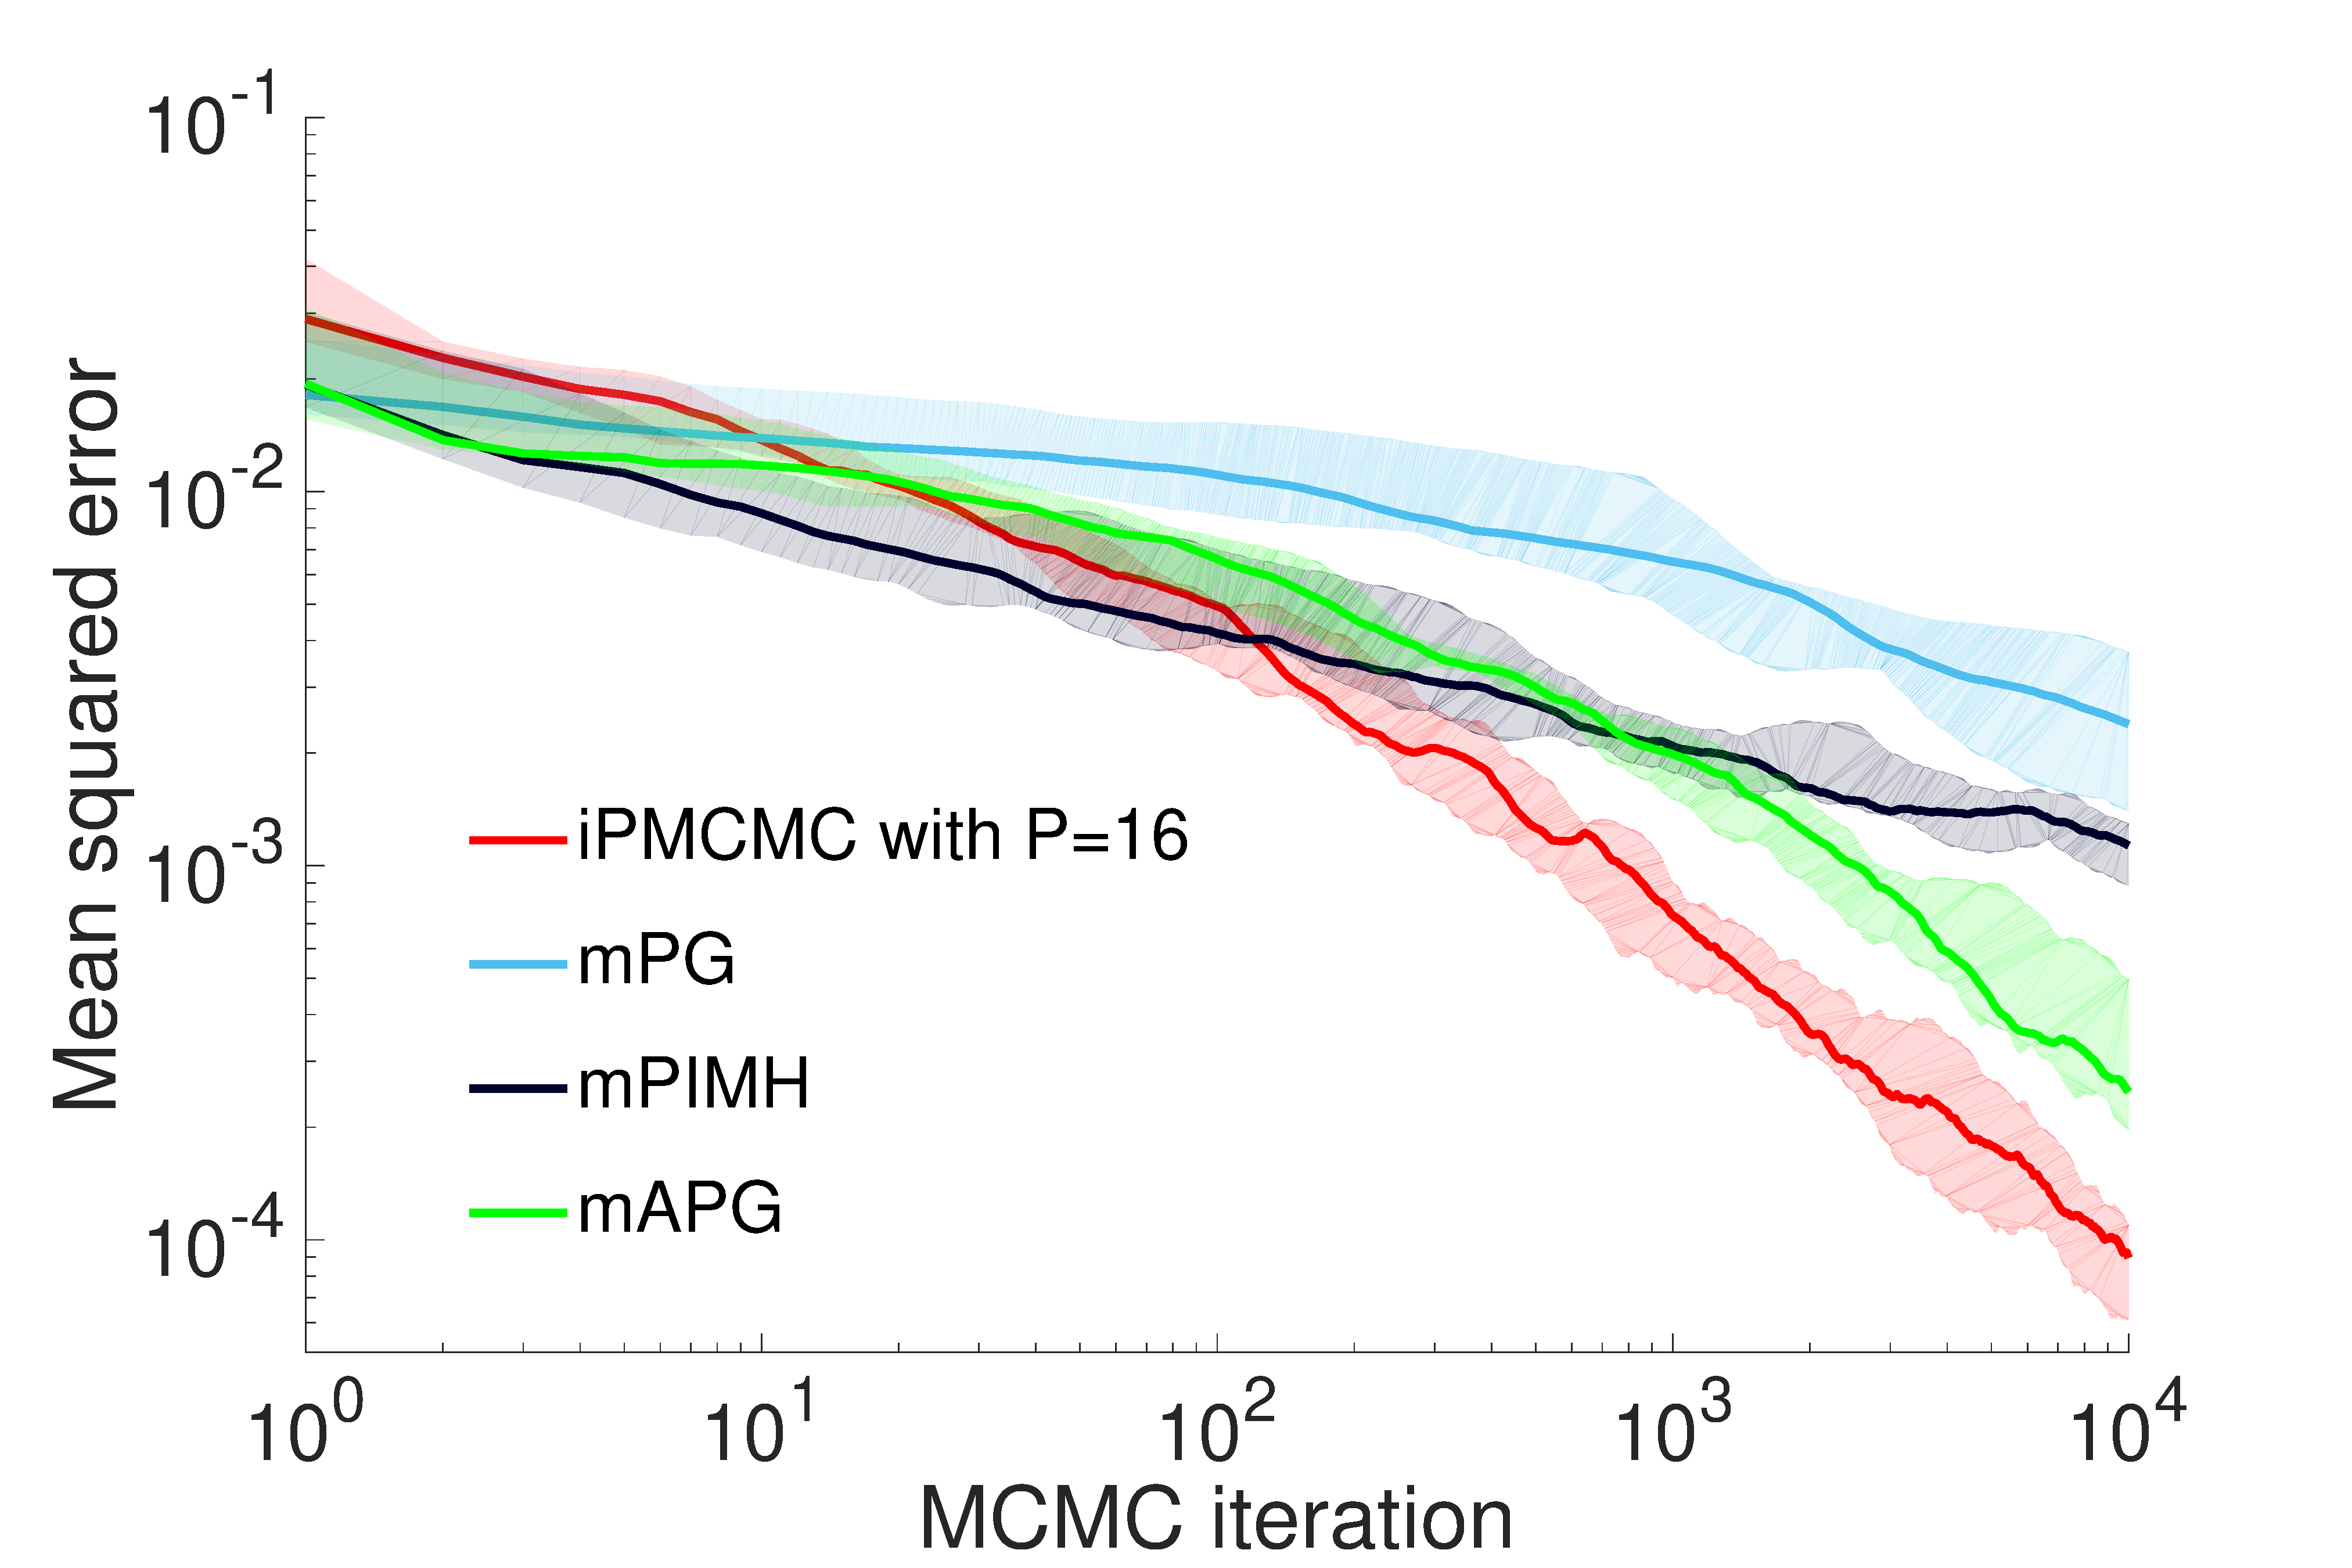
\includegraphics[width=0.98\textwidth]{mean_conv_lss}
		\caption{Convergence in mean for full sequence}
		\label{fig:meanConv}
	\end{subfigure}
	~  %add desired spacing between images, e. g. ~, \quad, \qquad, \hfill etc. 
	%(or a blank line to force the subfigure onto a new line)
	\begin{subfigure}[t]{0.49\textwidth}
		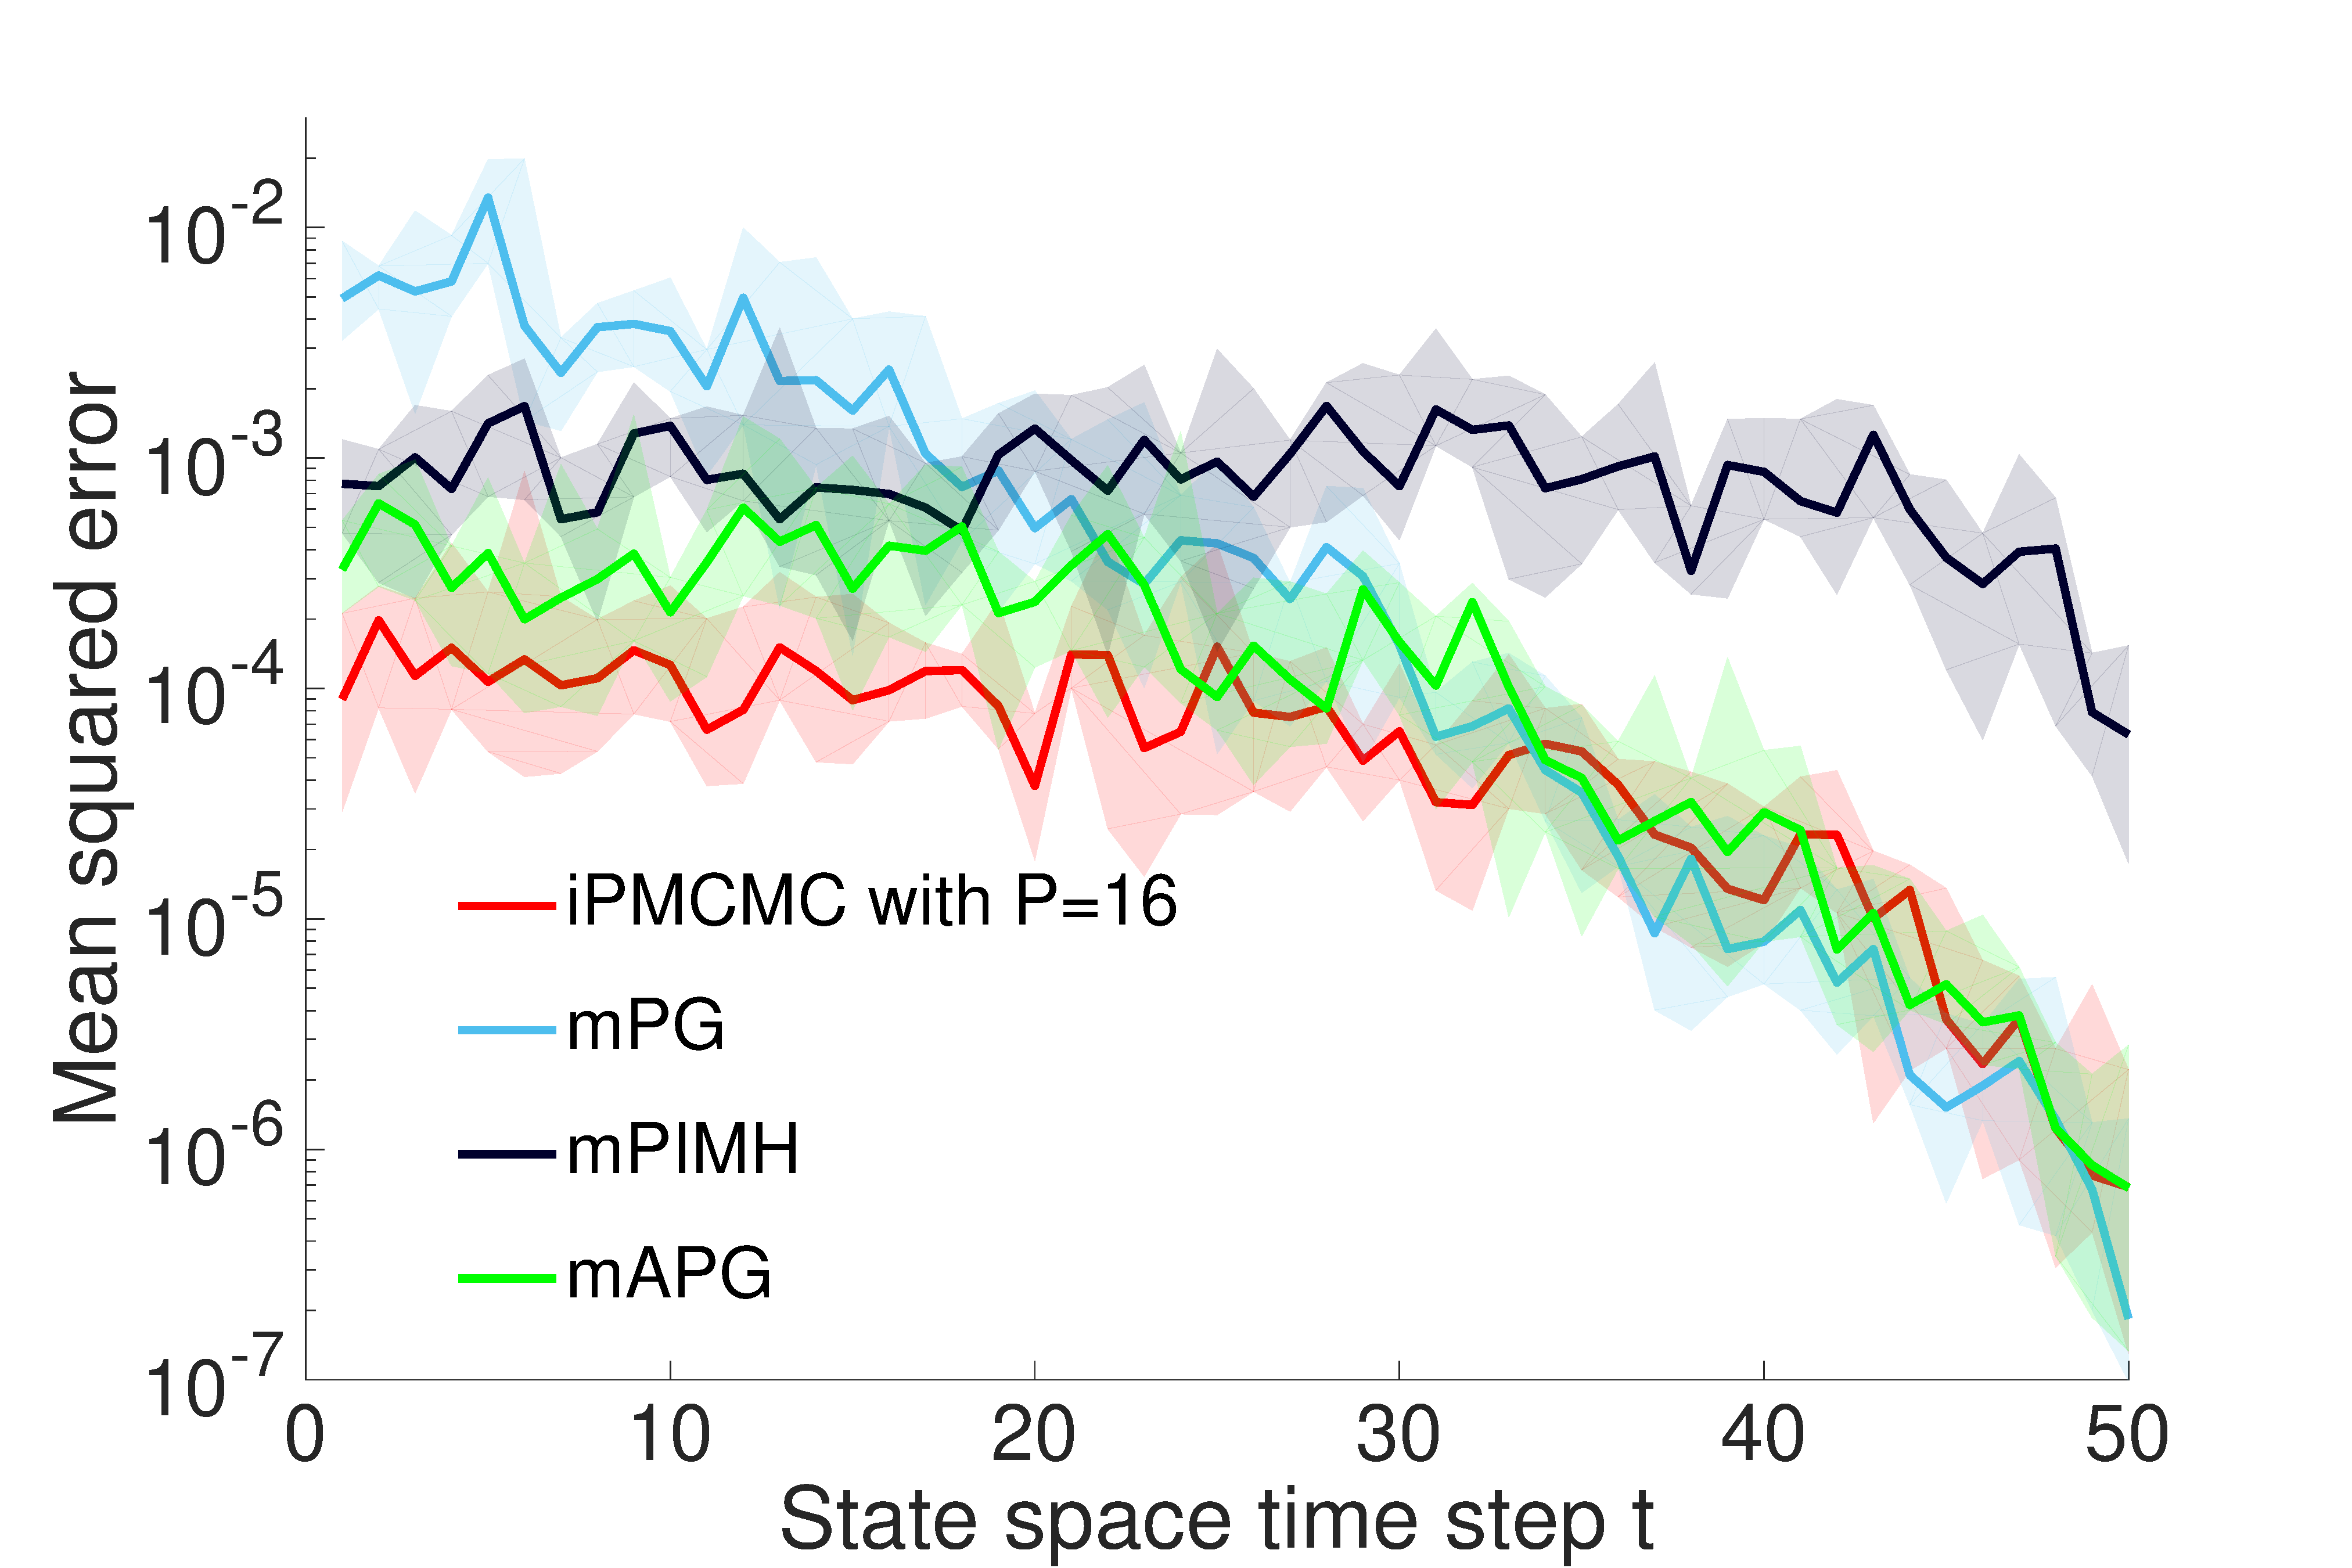
\includegraphics[width=0.98\textwidth]{mean_pos_lss}
		\caption{Final error in mean for latent marginals}
		\label{fig:meanPos}
	\end{subfigure}
	
	%	\begin{subfigure}[t]{0.49\textwidth}
	%		\includegraphics[width=\textwidth]{std_conv_lss}
	%		\caption{Convergence in standard deviation for full sequence}
	%		\label{fig:stdConv}
	%	\end{subfigure}
	%	~ %add desired spacing between images, e. g. ~, \quad, \qquad, \hfill etc. 
	%	%(or a blank line to force the subfigure onto a new line)
	%	\begin{subfigure}[t]{0.49\textwidth}
	%		\includegraphics[width=\textwidth]{std_pos_lss}
	%		\caption{Final error in standard deviation for latent marginals}
	%		\label{fig:stdPos}
	%	\end{subfigure}	
	\vspace{5pt}
	\caption{Mean squared error averaged over all dimensions and steps in the state sequence as a function of MCMC iterations (left) and mean squared error after $10^4$ iterations averaged over dimensions as function of position in the state sequence (right) for \eqref{eq:LGSS} with 50 time sequences.  The solid line shows the median error across the 10 tested synthetic datasets, while the shading shows the upper and lower quartiles.  Ground truth was calculated using the Rauch--Tung--Striebel smoother algorithm \cite{rauch1965maximum}. 
		\label{fig:groundTruth}}
\end{figure*}

Figure \ref{fig:meanConv} shows convergence (in MCMC iterations) in the estimate of the latent variable means to the ground-truth solution for iPMCMC and the benchmark algorithms.  It shows that iPMCMC comfortably outperforms the alternatives from around 200 iterations onwards, with only iPMCMC and mAPG demonstrating behaviour consistent with the Monte Carlo convergence rate, suggesting that mPG and mPIMH are still far from the ergodic regime.  Figure \ref{fig:meanPos} shows the same errors after $10^4$ MCMC iterations as a function of position in state sequence.  It demonstrates that iPMCMC outperformed all the other algorithms for the early stages of the state sequence, for which mPG performed particularly poorly. Toward the end of state sequence, iPMCMC, mPG and mAPG all gave similar performance, whilst that of mPIMH was significantly worse.

\begin{figure*}[t]
	\centering
	\begin{subfigure}[t]{0.49\textwidth}
		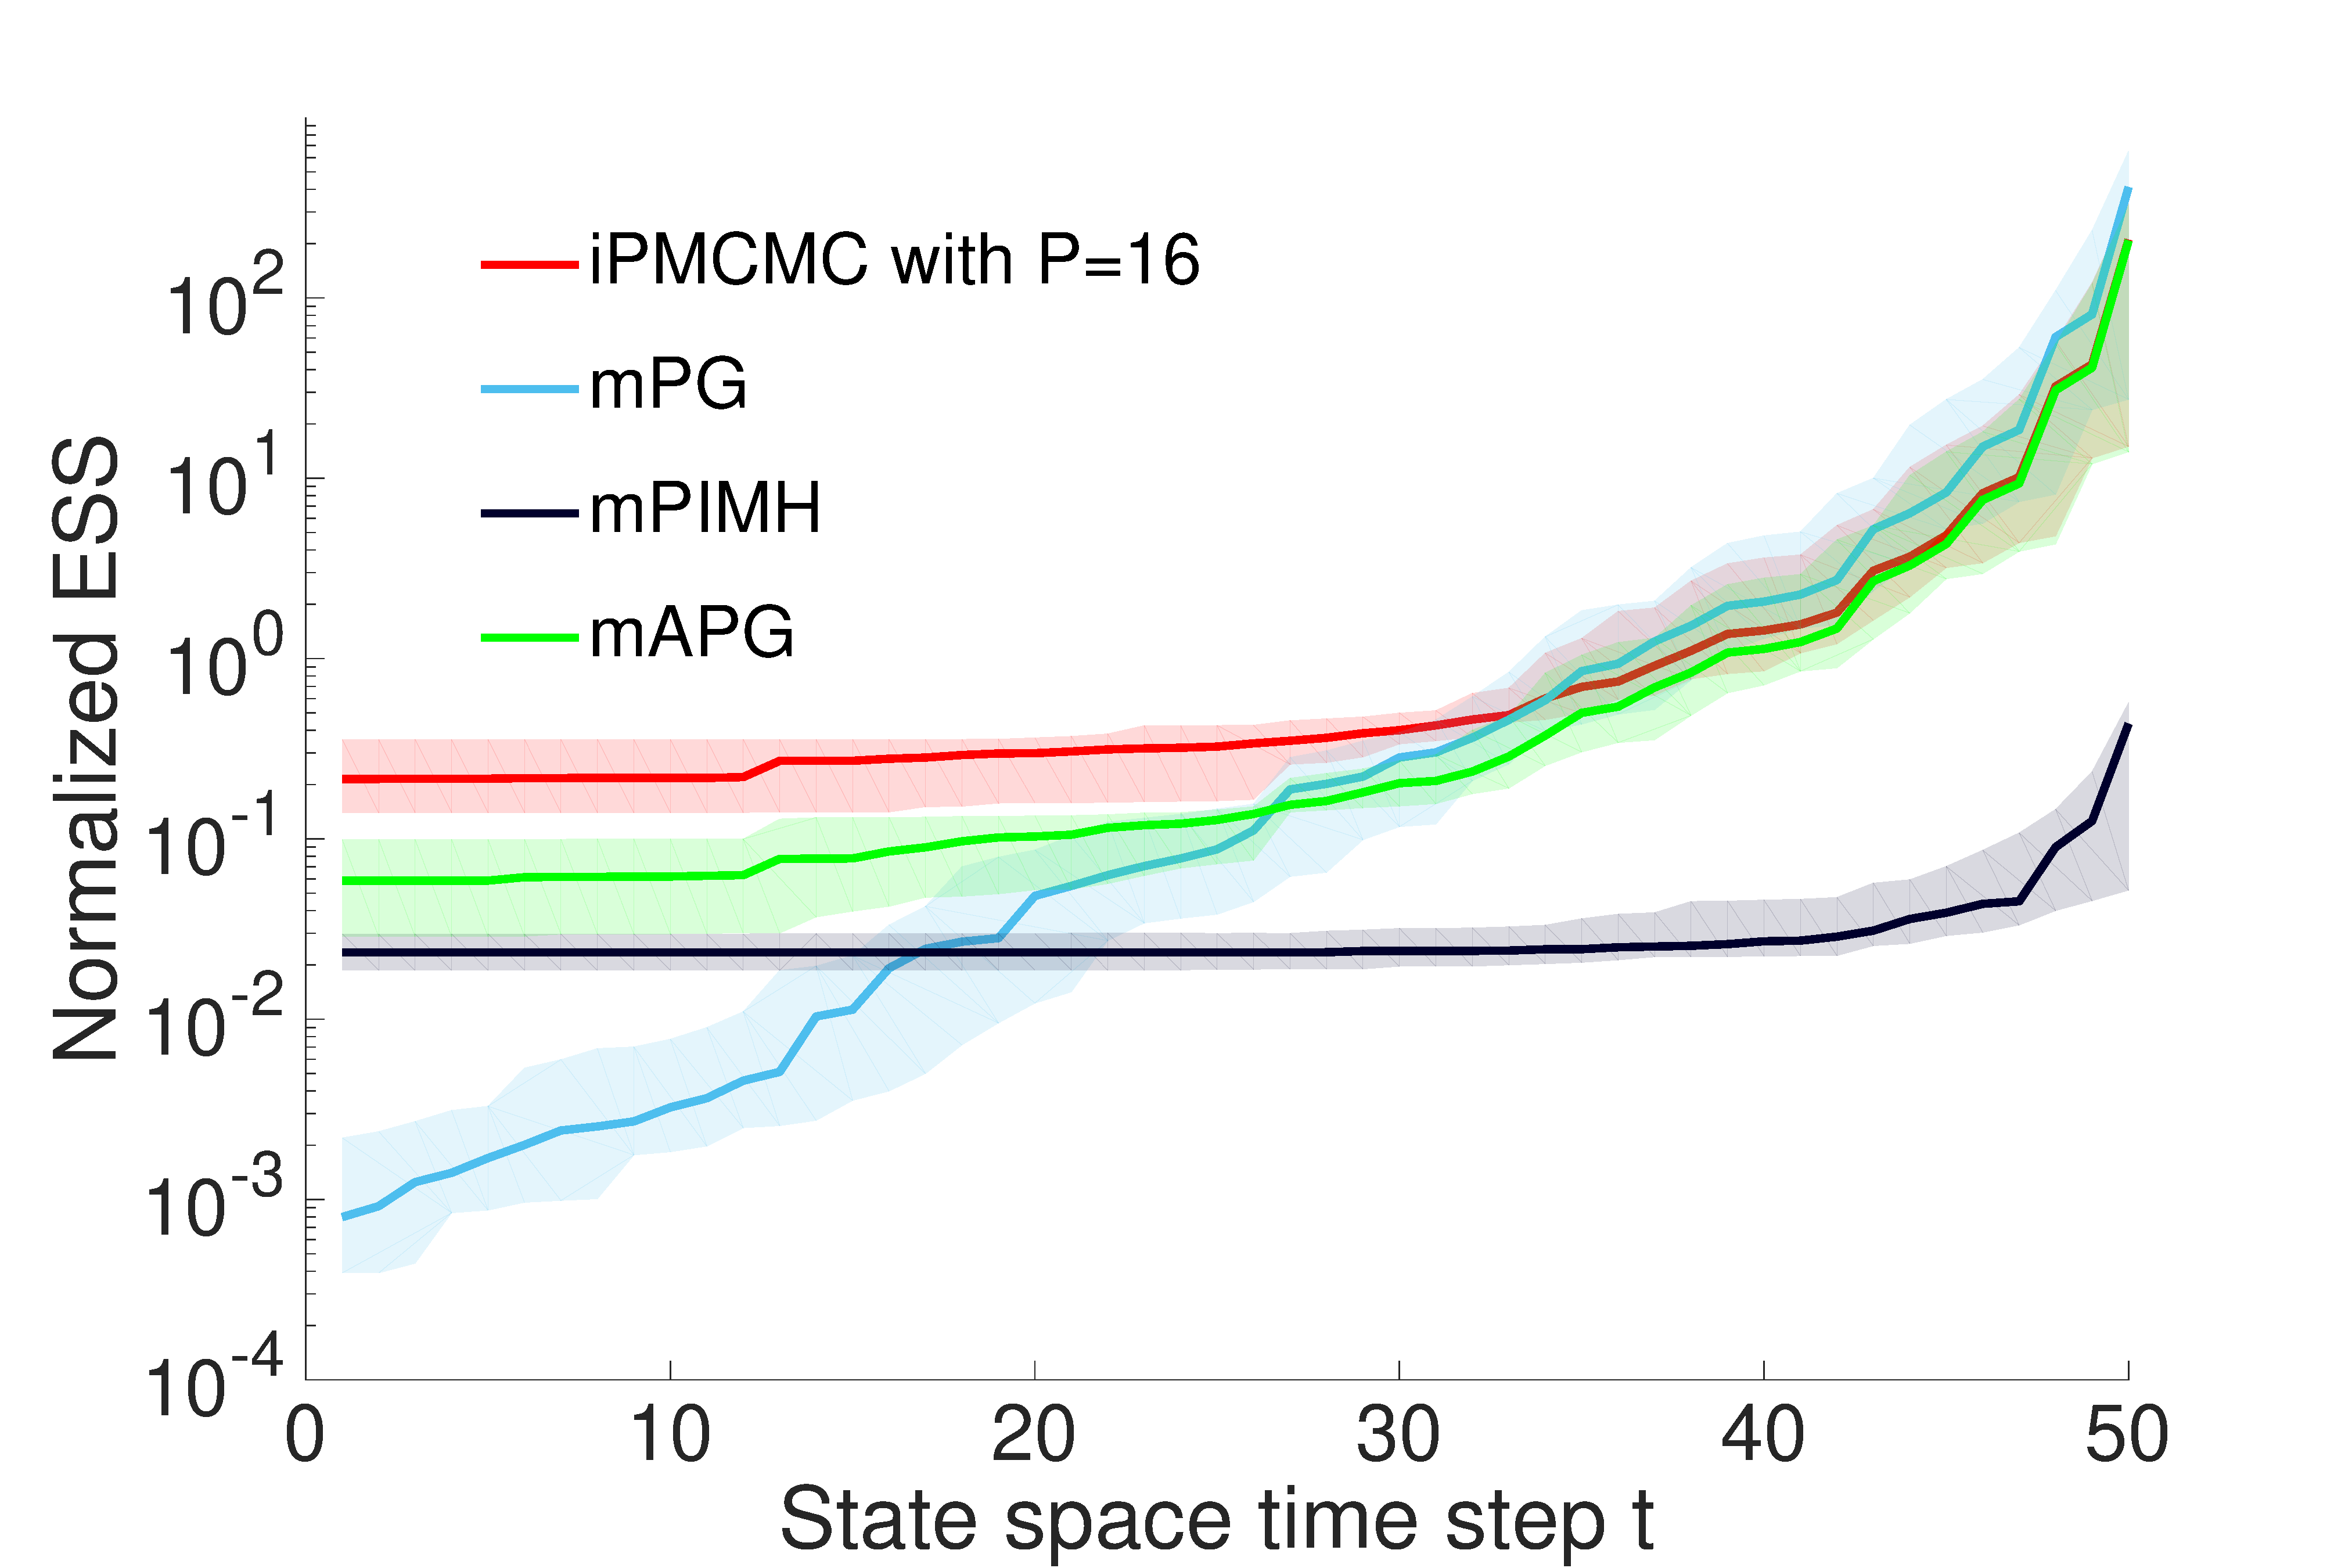
\includegraphics[width=\textwidth]{ess_lss}
		\caption{LGSSM}
	\end{subfigure}
	~ %add desired spacing between images, e. g. ~, \quad, \qquad, \hfill etc. 
	%(or a blank line to force the subfigure onto a new line)
	\begin{subfigure}[t]{0.49\textwidth}
		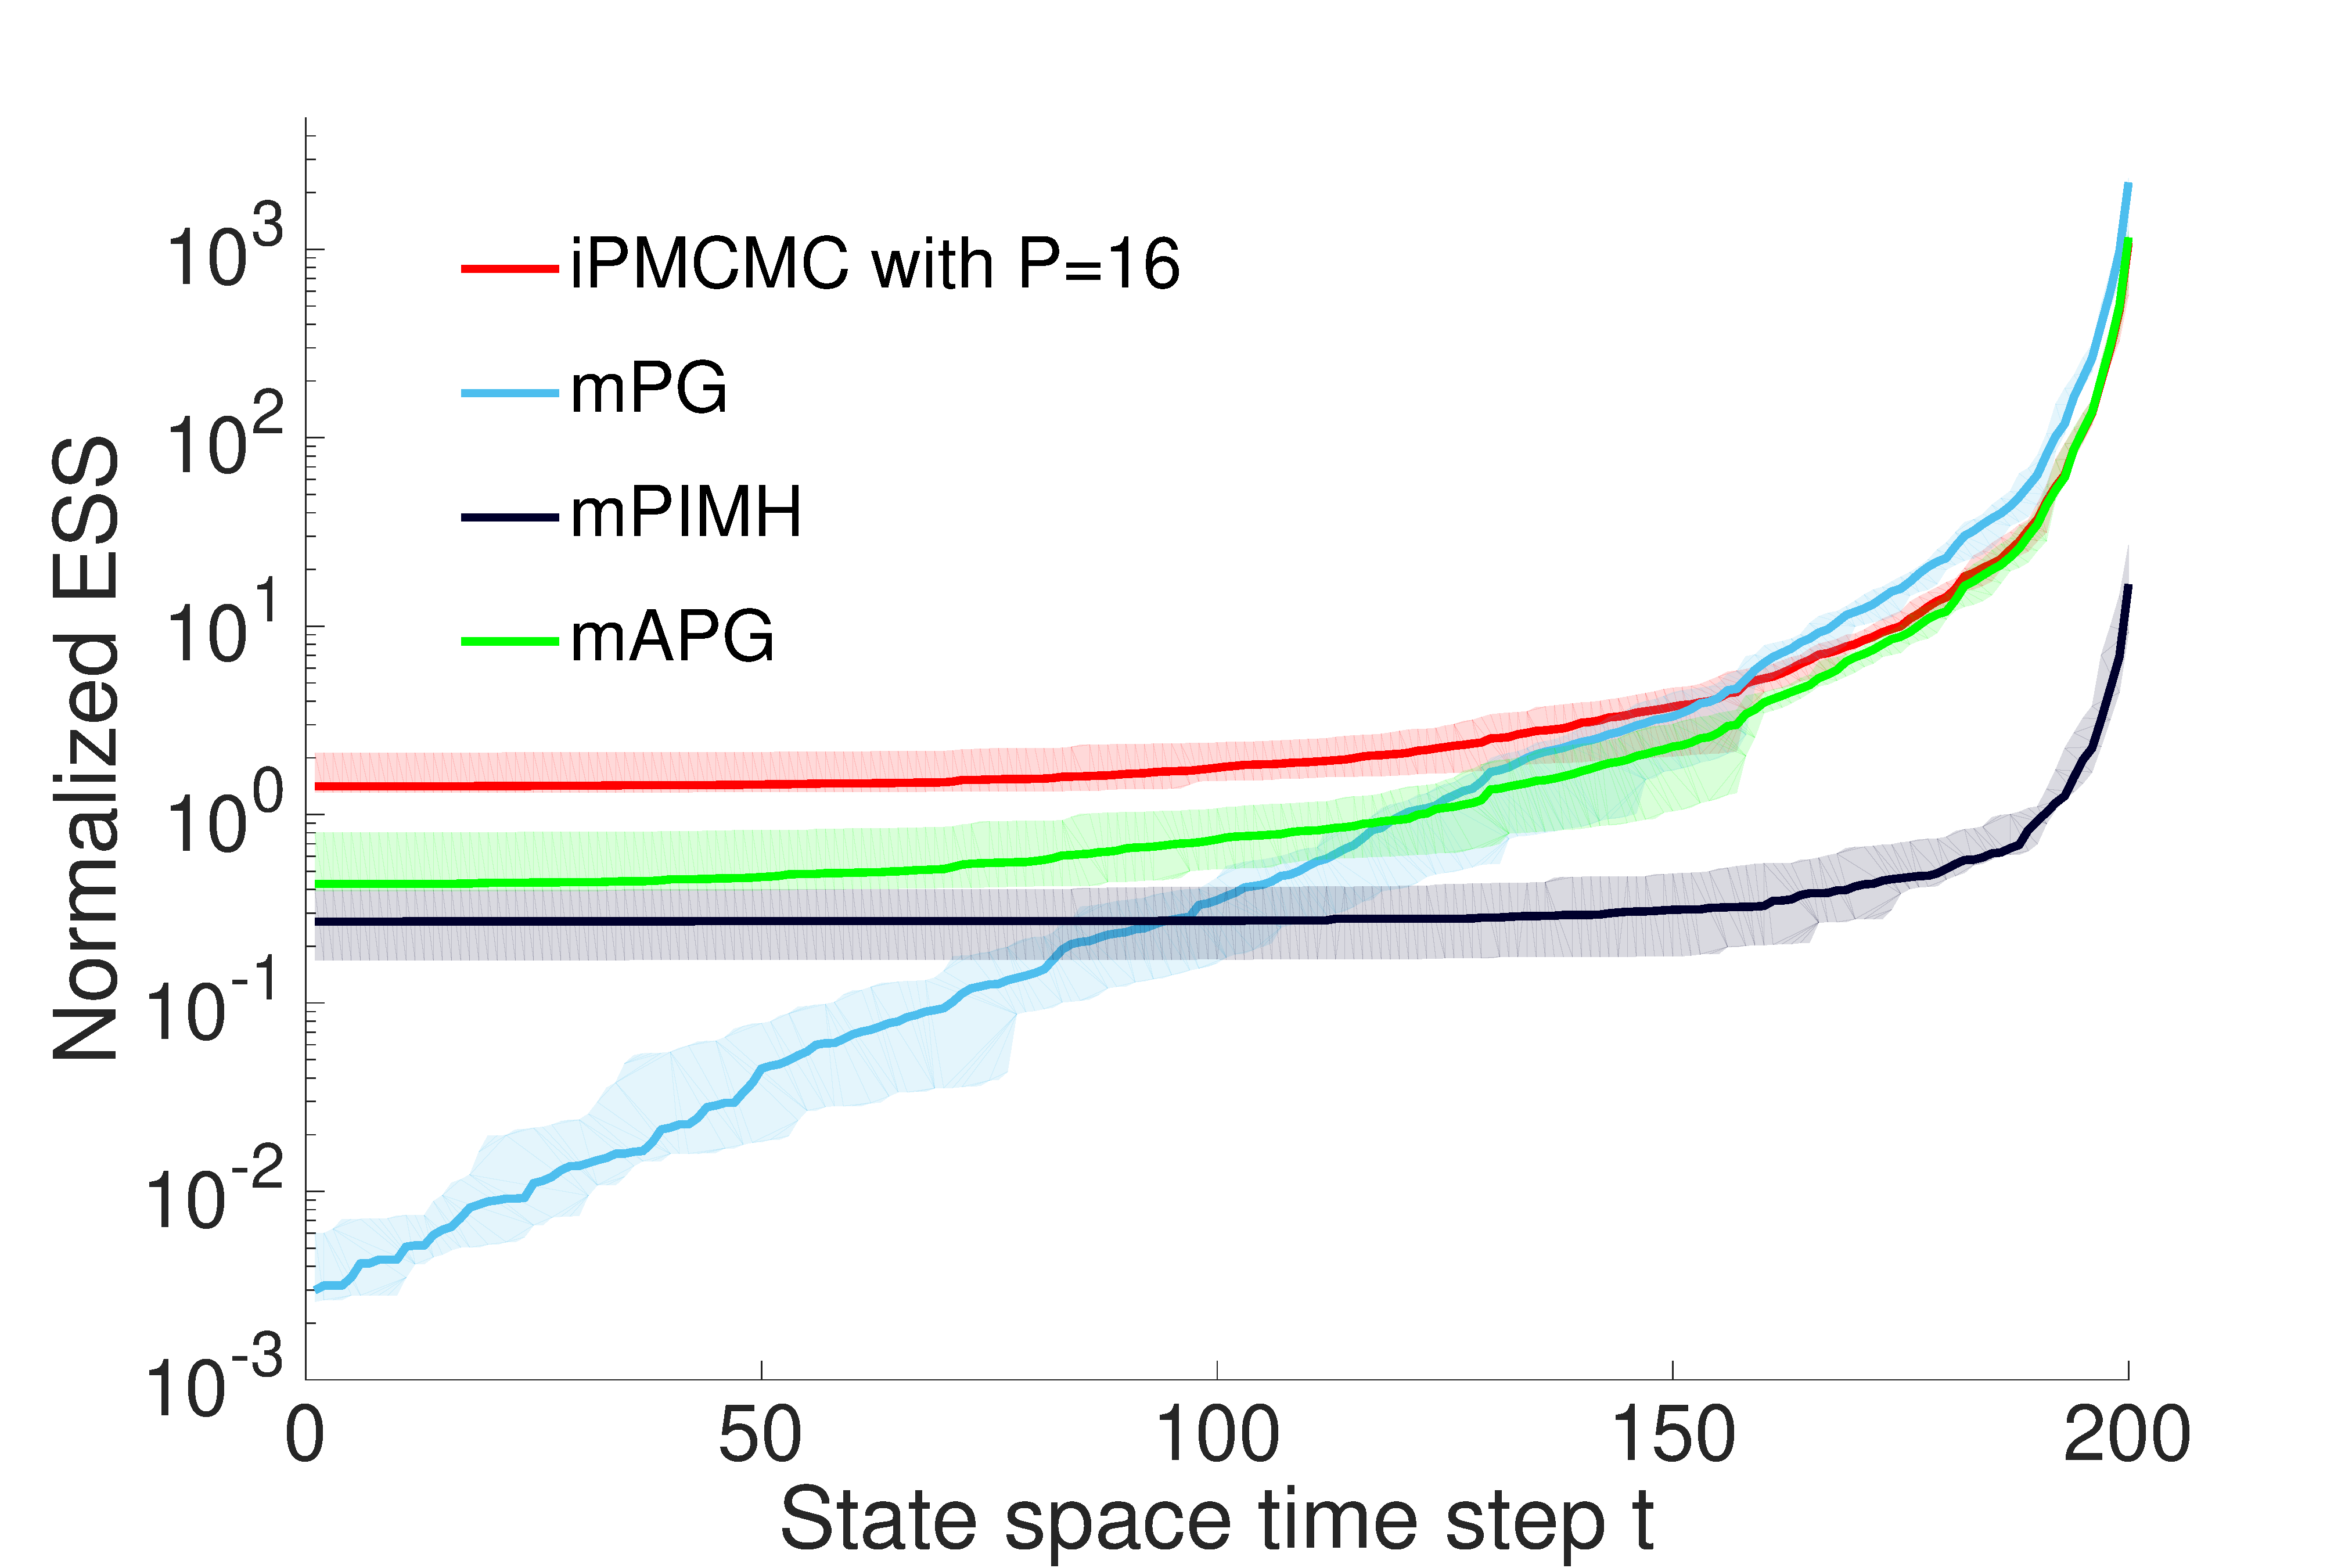
\includegraphics[width=\textwidth]{ess_nlss}
		\caption{NLSSM}
	\end{subfigure}
	\vspace{5pt}
	\caption{Normalized effective sample size  (NESS) for LGSSM (left) and NLSSM (right).
		\label{fig:ESS}}
	\vspace{-5pt}
\end{figure*}

\subsubsection{Nonlinear State Space Model}
\label{sec:nlss}

We next consider the one dimensional nonlinear state space model (NLSSM) considered by, among others, \citet{gordon1993novel,andrieuDH2010}
\begin{subequations}
	\label{eq:NLSS}
	\begin{align}
	x_1 & \sim \mathcal{N} \left(\mu, v^2\right) \label{eq:NLSSa} \displaybreak[0]\\
	x_t & = \frac{x_{t-1}}{2} + 25 \frac{x_{t-1}}{1+x_{t-1}^2} + 8 \cos \left(1.2t\right) + \delta_{t-1} \label{eq:NLSSb} \displaybreak[0]\\
	y_t & = \frac{{x_{t}}^2}{20} + \varepsilon_{t} \label{eq:NLSSc}
	\end{align}
\end{subequations}
where $\delta_{t-1} \sim \mathcal{N} \left(0, \omega^2\right)$ and $\varepsilon_{t} \sim \mathcal{N} \left(0, \sigma^2\right)$.  We set the parameters as $\mu = 0$, $v=\sqrt{5}$, $\omega = \sqrt{10}$ and $\sigma = \sqrt{10}$.  Unlike the LGSSM, this model does not have an analytic solution and therefore one must resort to approximate inference methods. 
% such as sampling.
Further, the multi-modal nature of the latent space makes full posterior inference over $x_{1:T}$ challenging for long state sequences. 

\begin{figure*}[t]
	\centering
	%\begin{subfigure}[t]{0.99\textwidth}
	\includegraphics[width=1\textwidth]{nlss_histograms_minus_190.pdf}
	%\end{subfigure}
	\caption{Histograms of generated samples at $t=1, 100, \text{ and } 200$ for a single dataset generated from \eqref{eq:NLSS} with $T=200$.  Dashed red line shows an approximate estimate of the ground truth, found by running a kernel density estimator on the combined samples from a small number of independent SMC sweeps, each with $10^7$ particles. \label{fig:nlssHists}}
	\vspace{-10pt}
\end{figure*}

To examine the relative mixing of iPMCMC we calculate an effective sample size (ESS) for different steps in the state 
sequence as described in Section~\ref{sec:inf:foundation:ess}, taking care to  condensed identical samples.  To be
precise, let
\begin{align*}
u_{t}^k \in \{x_{t,m}^{i}[r]\}^{i=1:N,r=1:R}_{m=1:M}, \quad \forall k \in 1 \dots K, \; t \in 1 \dots T
\end{align*} 
denote the unique samples of $x_t$ generated by all the nodes and sweeps of particular algorithm after $R$ iterations, where $K$ is the total number of unique samples generated.  The weight assigned to these unique samples, $v_t^{k}$, is given by the combined weights of all particles for which $x_t$ takes the value $u_{t}^k$:
\begin{align}
v_t^{k} = \sum_{r=1}^{R} \sum_{m=1}^{M} \sum_{i=1}^{N} \bar{w}_{t,m}^{i,r} \eta_{m}^{r} \delta_{x_{t,m}^{i}[r]}(u_{t}^{k})
\end{align}
where $\delta_{x_{t,m}^{i}[r]}(u_{t}^{k})$ is the Kronecker delta function and $\eta_{m}^{r}$ is a node weight.  For iPMCMC the node weight is given by as per the Rao-Blackwellized estimator described in Section~\ref{sec:part:ipmcmc:allparticles}. For mPG and mPIMH, $\eta_{m}^{r}$ is simply $\frac{1}{RM}$,
as samples from the different nodes are weighted equally in the absence of interaction. 
Finally we define our effective sample size as $\text{ESS}_t = \left(\textstyle\sum_{k=1}^K \left(v_t^{k}\right)^2\right)^{-1}$.
%\begin{align}
%\label{eq:ESS}
%\text{ESS}_t = \left(\textstyle\sum_{k=1}^K \left(v_t^{k}\right)^2\right)^{-1}.
%\end{align}

Figure \ref{fig:ESS} shows the ESS for the LGSSM and NLSSM as a function of position in the state sequence.  For this, we omit the samples generated by the initialization step as this SMC sweep is common to all the tested algorithms.  We further normalize by the number of MCMC iterations so as to give an idea of the rate at which unique samples are generated.  These show that for both models the ESS of iPMCMC, mPG and mAPG is similar towards the end of the space sequence, but that iPMCMC outperforms all the other methods at the early stages. The ESS of mPG was particularly poor at early iterations.  PIMH performed poorly throughout, reflecting the very low observed acceptance ratio of around $7.3\%$ on average. 
%The lack of Monte Carlo convergence rate appearing in Figure \ref{fig:meanConv} also suggests this acceptance ratio is yet to converge, with the value in the ergodic regime likely to be even lower.   

It should be noted that the ESS is not a direct measure of performance for these models.  For example, the equal weighting of nodes is likely to make the ESS artificially high for mPG, mPIMH and mAPG, when compared with methods such as iPMCMC that assign a weighting to the nodes at each iteration.  To acknowledge this, we also plot histograms for the marginal distributions of a number of different position in the state sequence as shown in Figure \ref{fig:nlssHists}.  These confirm that iPMCMC and mPG have similar performance at the latter state sequence steps, whilst iPMCMC is superior at the earlier stages, with mPG producing almost no more new samples than those from the initialization sweep due to the degeneracy.  The performance of PIMH was consistently worse than iPMCMC throughout the state sequence, with even the final step exhibiting noticeable noise.

%An important feature of the ESS is that it is equal to the total number of samples ($NRM$) if all the samples are unique and have the same weight, and is equal to $1$ if there is only single unique sample with non-zero weight. It should be noted that ESS is not a direct measure of performance in the context of distributed PMCMC methods. In particular it takes no account of the suitability of the weights assigned to samples, for example the equal weighting assigned to different chains for mPG and mPIMH mean they will always have a higher ESS for a particle sweep \brooks{clarify ``particle sweep''?} than a iPMCMC sweep generating the same samples, regardless of whether this equal weighting gives a better approximation to the true posterior. \fredrik{I did not quite understand the last sentence.}


\section{Discussion and Future Work}
\label{sec:disc}

% !TEX root = ../main.tex

\chapter{Challenges, Criticisms, and Future Directions}
\label{chp:discussion}

\begin{itemize}
	\item Relationships with ABC
	\item Reinvention of priors in deep learning by generating data
	\item Is amortization just a learning a different decomposition of the joint 
	$p(\theta | \mathcal{D}_1)p(\mathcal{D}_2|\theta)$ that shifts more to the
	prior to make inference easier?  Does it actually implicitly define a different
	joint distribution that is otherwise difficult to express or is it just proposal
	adaptation as Tuan Anh's paper says.
	\item Randomness vs no randomness - blog post for Michi
	\item Packages for experimental design -- point heavily to the work with Ben.
	\item Sort out PPS vs PPL and PPS vs PPSs
	\item Add reference somewhere to the paper with Andrew
\end{itemize}

\section{Do we need Random Numbers?}
	
Random numbers are a fundamental tool in the arsenal of all the mathematical sciences, especially in the realm of 
probabilistic numerics.  From basic cross-validation to advanced MCMC methods, randomness is at the core of 
many of our most prevalent and highest performance algorithms.  In his related post, Michael will 
try to convince you why we should eventually try and do away this randomness; here I will do my best to explain why
\texttt{if(rand<1-$\varepsilon$)\{we should not\}}.

My argument can be broken down into four main reasons that we need, and always will need, random numbers:
\begin{enumerate}
	\item Speed and simplicity - sometimes even if there if there is the information available to improve a computation, 
	uncovering or incorporating that information in a principled manner may require substantially more computational 
	power than not doing so.
	\item Honesty and reliability - the alternative to randomness is almost always approximation, introducing bias 
	and an error whose uncertainty is inherently subjective.
	\item Compossibility - methods such as Monte Carlo are ambivalent to how the samples are to be used, creating 
	a scalable ability to modularize, compose and reuse.  Non-compossible systems, on the other hand, are doomed to fail
	for large frameworks through the curse of repeated nested of estimators~\citep{rainforth2017pitfalls}
	\item Lack of repeatability - though it is always convenient when an experiment is repeatable, systematically 
	returning the same incorrect answer is far more dangerous.
\end{enumerate}
Of these, the speed and simplicity argument is perhaps the most commonly used to support the use of random 
numbers and is certainly a core reason for their prevalence.  However, I believe it is the other three, and in 
particular the honesty of random numbers, that is most critical for why random numbers are, will remain to be, 
fundamental to numerical computation.  All of these arguments are related to the following principle:

\emph{Once we have imparted all possible information upon a system, we must treat what is left as truly 
	stochastic or introduce bias.}

In other words, imagine we can construct a problem in a manner that utilizes all available prior information,
both in terms of the model and in how best to solve the model.
Any remaining uncertainty is now, at least for all practical purposes, inherent to the problem and so any
further attempt to remove randomness from the system is indirectly adding in further prior information we
did not want to impart.  Furthermore, when things we kept random, we can gauge the error in our approximation
or the level of our uncertainty by simply rerunning the system.  As soon as we replace this with an approximation
or fix the random number seed, we lose calibration of the uncertainty in our estimate because we can estimate the variance
resulting from randomness, but typically not the bias resulting from approximation.

Putting our frequentist hat on for the moment, then the notion of doing away with randomness is scary.
Frequentist statistics is all about \emph{repeatability} and focuses on the fact that any data we collect is random
in a many-worlds point of view,
because even with the same ground-truth underlying generative process, the inherent randomness
of the universe (or at least effective randomness if you have philosophical objects to this) means that multiple possible
datasets \emph{could} have been generated.  Regardless of your philosophical position on the Bayesian vs frequentist divide,
there are many times when such a frequentist approach is absolutely essential from a practical viewpoint.  For example, in medical tasks we need
to make sure that our confidence intervals are actually correct when we repeat a procedure -- we need guarantees on
their \emph{calibration}.  This simply is not possible in a Bayesian framework as by its very nature it presumes the data
is fixed and thus permits no concept of repetition.  Once we realize that we sometimes need to take a frequentist
approach, the need for randomness becomes obvious, as in the frequentist framework probability originates only
through random variables.  In other words, as powerful as the Bayesian framework is, it is inherently optimistic and subjective
(e.g. there are always unknown unknowns), and as such it can never really be the whole story.  If we try and
do away with randomness completely it is impossible to be objective -- we have to choose our approximation, sometimes
in an arbitrary fashion (e.g. by setting the random number seed) -- and so we can never provide properly calibrated confidence 
intervals that are not prone to subjective interpretation.

This honesty of Monte Carlo goes beyond specific applications.  One of its most powerful consequences is the compossibility
of Monte Carlo estimates: give a sample from a marginal, I can generate a valid sample of the joint by sampling from the
conditional.  Similarly, if I have samples from a joint, I also have samples from the marginal distributions.  This behavior
is essential when composing different components into a greater system as one can ensure each component takes in
samples as inputs and outputs corresponding samples as output that can be used by the next process in the pipeline.
If we instead make some deterministic approximation at each stage, we flaunt the flaw of averages and our biases
will conflagulate to give a result that might be substantially different to the truth.  Sticking with unbiased Monte Carlo estimation
(e.g. using importance sampling or sequential Monte Carlo~\citep{doucet2009tutorial}) then although it is of course possible that our 
variance will explode, we at least know that if our estimate has a poor accuracy.  If we do away with randomness,
we might generate large errors without even knowing we have.

This lack of repeatability is actually an essential advantage of Monte Carlo.  It is better for a system to give you
a different wrong answer each time it is queried than to always give the same wrong answer, particularly if the average
of the different answers is in fact the truth, as is often the case.  When we write scientific papers we run our experiments
multiple times to show the variability in the results.  Systems that always give the same answer and instead return
a single subjective uncertainty estimate (e.g. a Gaussian process) are not generally trustworthy because there is no
true calibration or sense of whether the experimenter simply got lucky with a system that does not actually work well
in practice.  Furthermore, such a setting it very open to intentional or unintentional abuse.  If we fix our randomness
a priori and then adapt our algorithm until it works, we may well simply be over-fitting to what works best for that
random number seed or approximation.  It horrifies me that some people fix their random number seeds when 
tunning or improving an algorithm and I expect that this practice has actually led to a plethora of statistically incorrect
results.  If we want to maintain scientific integrity then we have to report results on experiments that have not been
tested during the design of our algorithm and which are tested with multiple different choices for arbitrary or subjective
decisions, to show that those results are actually stable and representative.  If we do away with randomness, we lose, or at the very least
seriously hamper, this ability to repeat experiments in an objective manner.

To summarize, we need randomness because we do not know everything.  In the Bayesian framework we place distributions
on what we are not sure about to reflect this lack of knowledge.  A key part of this process is acknowledging that once we
have done this, what is left is random.  After all, this uncertainty is where the Bayesian definition of probability actually comes
from and what does it mean to have probability without randomness?  Yes we might be able to impart more knowledge on
problems that we currently do, such as by decorrelating our samples, but there always become a point where we have
imparted everything we know, after which what is left is truly random by the Bayesian definition of
probability.  If we go outside the Bayesian framework, the need for randomness becomes even more pronounced.  In
frequentist settings even our data is a random variable and probability is defined through variations in repeating an
experiment.  In short, regardless of whether we take a Bayesian or frequentist viewpoint, arguing for the 
removal of all randomness from our system is tantamount to arguing that we should do away with probability
theory entirely.

\newpage

\appendix

\section{Program Transformations in Detail}
\label{sec:program-transformations}
% !TEX root = bopp.tex

In this section we give a more detailed and language specific description of our program transformations, code for which can be found at \href{http://www.github.com/probprog/bopp}{\url{http://www.github.com/probprog/bopp}}. %We will refer to the code in explaining the implementation of program transformations for BOPP.

\subsection{Anglican}
Anglican is a probabilistic programming language integrated into Clojure (a dialect of Lisp) and inherits most of the corresponding syntax. Anglican extends Clojure with the special forms \sample and \observe \citep{tolpin2015probabilistic}.  
Each random draw in an Anglican program corresponds to a \sample  call, which can be thought of as a term in the prior. 
Each \observe statement applies weighting to a program trace and thus constitutes a term in the likelihood.
Compilation of an Anglican program, performed by the macro \lsi{query}, corresponds to transforming the code into a variant of continuation-passing style (CPS) code, which results in a function that can be executed using a particular inference algorithm.

Anglican program code is represented by a nested list of expressions, symbols, non-literals for contructing data structures (e.g. \lsi{[...]} for vectors), and command dependent literals (e.g. \lsi{[...]} as a second argument of a \lsi{let} statement which is used for binding pairs).  In order to perform program transformations, we can recursively traverse this nested list which can be thought of as an abstract syntax tree of the program.

Our program transformations also make use of the Anglican forms \lsi{store} and \lsi{retrieve}.  These allow storing any variable in the probabilistic program's execution trace in a state which is passed around during execution and from which we can retrieve these stored values.  The core use for this is to allow the outer query to return variables which are only locally scoped.

To allow for the early termination that will be introduced in Section \ref{sec:bopp-supp/early-term}, it was necessary to add a mechanism for non-local returns to Anglican.  Clojure supports non-local returns only through Java exception handling, via the keywords {\bf\ttfamily\color{cyan} try}~{\bf\ttfamily\color{cyan}throw},~{\bf\ttfamily\color{cyan}catch} and {\bf\ttfamily\color{cyan}finally}.  Unfortunately, these are not currently supported by Anglican and their behaviour is far from ideal for our purposes.  In particular, for programs containing nested {\bf\ttfamily\color{cyan}try} statements, throwing to a particular {\bf\ttfamily\color{cyan}try} in the stack, as opposed to the most recently invoked, is cumbersome and error prone.
%
%Firstly, return values are stored within exceptions which is cumbersome and can cause issues in debugging.  Secondly, it is difficult to control the point of return.  For example, imagine we wish to return from the query itself and so wrap the original query in a {\bf\ttfamily\color{cyan}try-catch} block.  Na\"{i}vely throwing might now cause us to return to an unexpected point if the original query already contained a {\bf\ttfamily\color{cyan}try-catch} block.  Thus controlling the exact return point would require a careful and error-prone mechanism based on custom exception types and catches.

We have instead, therefore, added to Anglican a non-local return mechanism based on the Common Lisp control form \lsi{catch/throw}.  This uses a \emph{catch tag} to link each \lsi{throw} to a particular \lsi{catch}.  For example
\begin{lstlisting}[basicstyle=\footnotesize\ttfamily]
(catch :tag
  (when (> a 0)
    (throw :tag a))
  0)
\end{lstlisting}
is equivalent to \lsi{(max a 0)}.  More precisely, \lsi{throw} has syntax \lsi{(throw tag value)} and will cause the \lsi{catch} block with the corresponding \lsi{tag} to exit, returning \lsi{value}.   If a \lsi{throw} goes uncaught, i.e. it is not contained within a \lsi{catch} block with a matching tag, a custom Clojure exception is thrown.

%To allow for the early termination discussed in Section \ref{sec:bopp-supp/early-term}, it was necessary to add one new primitive to Anglican, namely \lsi{return} with syntax \lsi{(return return-val)}.  At a high level, \lsi{return} causes the query to terminate, returning \lsi{return-val}.  This is done by, during runtime of the CPS compiled code, returning a Clojure record \lsi{->result} containing \lsi{return-val} instead of a valid program continuation, causing the query execution to terminate and return the required value.

\subsection{Representations in the Main Paper}
\label{sec:bopp-supp/main-paper-rep}

In the main paper we presented the code transformations as static transformations as shown in Figure~\ref{fig:bopp_overview}.  Although for simple programs, such as the given example, these transformations can be easily expressed as static transformations, for more complicated programs it would be difficult to actually implement these as purely static generic transformations in a higher-order language.  Therefore, even though all the transformations dynamically execute as shown at runtime, in truth, the generated source code for the prior and acquisition transformations varies from what is shown and has been presented this way in the interest of exposition.  Our true transformations exploit \lsi{store}, \lsi{retrieve}, \lsi{catch} and \lsi{throw} to generate programs that dynamically execute in the same way at run time as the static examples shown, but whose actual source code varies significantly.

\subsection{Prior Transformation}
\label{sec:bopp-supp/prior-transformations}
The prior transformation recursively traverses the program tree and applies two local transformations.  
Firstly it replaces all \observe statements by \lsi{nil}.  
As \observe statements return \lsi{nil}, this trivially preserves the generative model of the program, but the probability of the execution changes. 
Secondly, it inspects the binding variables of \lsi{let} forms in order to modify the binding expressions for the optimization variables, as specified by the second input of \defopt, asserting that these are directly bound to a \sample statement of the form \texttt{(\sample dist)}.
The transformation then replaces this expression by one that stores the result of this sample in Anglican's \lsi{store} before returning it.
Specifically, if the binding variable in question is \lsi{phi-k}, then the original binding expression \lsi{(sample dist)} is transformed into
% \begin{figure}
    \begin{lstlisting}[basicstyle=\footnotesize\ttfamily]
(let [value (sample dist)]
  ;; Store the sampled value in Anglican's store
  (store OPTIM-ARGS-KEY
         'phi-k
         value)
  value)
    \end{lstlisting}
%     \caption{}
%     \label{fig:prior-1}
% \end{figure}

After all these local transformation have been made, we wrap the resulting query block in a \lsi{do} form and append an expression extracting the optimization variables using Anglican's \lsi{retrieve}.  This makes the optimization variables the output of the query.  Denoting the list of optimization variable symbols from \defopt as \lsi{optim-args} and the query body after applying all the above location transformations as \dots, the prior query becomes
% \begin{figure}
    \begin{lstlisting}[basicstyle=\footnotesize\ttfamily]
(query query-args
  (do
    ...
    (map (fn [x] (retrieve OPTIM-ARGS-KEY x))
       optim-args)))
    \end{lstlisting}
%     \caption{}
%     \label{fig:prior-3}
% \end{figure}
Note that the difference in syntax from Figure~\ref{fig:bopp_overview} is because \lsi{defquery} is in truth a syntactic sugar allowing users to bind \lsi{query} to a variable.  As previously stated, \lsi{query} is macro that compiles an Anglican program to its CPS transformation.  An important subtlety here is that the order of the returned samples is dictated by \lsi{optim-args} and is thus independent of the order in which the variables were actually sampled, ensuring consistent inputs for the BO package.

We additionally add a check (not shown) to ensure that all the optimization variables have been added to the store, and thus sampled during the execution, before returning.  This ensures that our assumption that each optimization variable is assigned for each execution trace is satisfied.

\subsection{Acquisition Transformation}
\label{sec:bopp-supp/acq-transformations}
The acquisition transformation is the same as the prior transformation except we append the acquisition function, \lsi{ACQ-F}, to the inputs and then \observe its application to the optimization variables before returning.
The acquisition query is thus
% \begin{figure}
    \begin{lstlisting}[basicstyle=\footnotesize\ttfamily]
(query [query-args ACQ-F]
  (do
    ...
    (let [theta (map (fn [x] (retrieve OPTIM-ARGS-KEY x))
                      optim-args)]
      (observe (factor) (ACQ-F theta))
      theta)))
    \end{lstlisting}
%     \caption{}
%     \label{fig:acq-1}
% \end{figure}

\subsection{Early Termination}
\label{sec:bopp-supp/early-term}
To ensure that \lsi{q-prior} and \lsi{q-acq} are cheap to evaluate and that the latter does not include unnecessary terms which complicate the optimization, we wish to avoid executing code that is not required for generating the optimization variables.
Ideally we would like to directly remove all such redundant code during the transformations.
However, doing so in a generic way applicable to all possible programs in a higher order language represents a significant challenge.
Therefore, we instead transform to programs with additional early termination statements, triggered when all the optimization variables have been sampled.  
Provided one is careful to define the optimization variables as early as possible in the program (in most applications, e.g. hyperparameter optimization, they naturally occur at the start of the program), this is typically sufficient to ensure that the minimum possible code is run in practise.

To carry out this early termination, we first wrap the query in a \lsi{catch} block with a uniquely generated tag.  We then augment the transformation of an optimization variable's binding described in Section~\ref{sec:bopp-supp/prior-transformations} to check if all optimization variables are already stored, and invoke a \lsi{throw} statement with the corresponding tag if so.  Specifically we replace relevant binding expressions \lsi{(sample dist)} with
% \begin{figure}
    \begin{lstlisting}[basicstyle=\footnotesize\ttfamily]
(let [value (sample dist)]
  ;; Store the sampled value in Anglican's store
  (store OPTIM-ARGS-KEY
         'phi-k
         value)
  ;; Terminate early if all optimization variables are sampled
  (if (= (set (keys (retrieve OPTIM-ARGS-KEY)))
         (set optim-args))
    (throw BOPP-CATCH-TAG prologue-code)
    value))
    \end{lstlisting}
%     \caption{}
%     \label{fig:early-termination}
% \end{figure}
where \lsi{prologue-code} refers to one of the following expressions depending on whether it is used for a prior or an acquisition transformation
% \begin{figure}
    \begin{lstlisting}[basicstyle=\footnotesize\ttfamily]
;; Prior query prologue-code
(map (fn [x] (retrieve OPTIM-ARGS-KEY x))
             optim-args)

;; Acquisition query prologue-code
(do
  (let [theta (map (fn [x] (retrieve OPTIM-ARGS-KEY x))
                    optim-args)]
  (observe (factor) (ACQ-F theta))
  theta))
    \end{lstlisting}
%     \caption{}
%     \label{fig:early-termination-2}
% \end{figure}

We note that valid programs for both \lsi{q-prior} and \lsi{q-acq} should always terminate via one of these early stopping criteria and therefore never actually reach the appending statements in the \lsi{query} blocks shown in Sections \ref{sec:bopp-supp/prior-transformations} and \ref{sec:bopp-supp/acq-transformations}.  As such, these are, in practise, only for exposition and error catching.

\subsection{Marginal/MMAP Transformation}
The marginal transformation inspects all \lsi{let} binding pairs and if a binding variable \lsi{phi-k} is one of the optimization variables, the binding expression \lsi{(sample dist)} is transformed to the following
% \begin{figure}
    \begin{lstlisting}[basicstyle=\footnotesize\ttfamily]
(do (observe dist phi-k-hat)
    phi-k-hat)
    \end{lstlisting}
%     \caption{}
%     \label{fig:marg-1}
% \end{figure}
corresponding to the \lsi{observe<-} form used in the main paper.

\subsection{Error Handling}
During program transformation stage, we provide three error-handling mechanisms to enforce the restrictions on the probabilistic programs described in Section~\ref{sec:problem}.
\begin{enumerate}
    \item We inspect \lsi{let} binding pairs and throw an error if an optimization variable is bound to anything other than a \sample statement.
    \item We add code that throws a runtime error if any optimization variable is assigned more than once or not at all.
    \item We recursively traverse the code and throw a compilation error if \sample statements of different base measures are assigned to any optimization variable.  At present, we also throw an error if the base measure assigned to an optimization variable is unknown, e.g. because the distribution object is from a user defined \lsi{defdist} where the user does not provide the required measure type meta-information.
\end{enumerate}


\section{Problem Independent Gaussian Process Hyperprior}
\label{sec:app:hyperprior}

% !TEX root = bopp.tex

Remembering that the domain scaling introduced in Section~\ref{sec:domain} means that both the input and outputs of the GP are taken to vary between $\pm1$, we define the problem independent GP hyperprior as $p(\alpha)=p(\sigma_n)p(\sigma_{3/2})p(\sigma_{5/2})\prod_{i=1}^{D}p(\rho_i)p(\varrho_i)$ where
\begin{subequations}
	\begin{align}
	\label{eq:hyperPriorDef}
	\log \left(\sigma_n\right) & \sim \mathcal{N} \left(-5,2\right) \\
	\log\left(\sigma_{3/2}\right) & \sim \mathcal{N} \left(-7,0.5\right)\\
	\log\left(\sigma_{5/2}\right) & \sim \mathcal{N} \left(-0.5,0.15\right)\\
	\log \left(\rho_i\right) & \sim \mathcal{N} (-1.5,0.5) \quad \forall i \in \{1,\dots,D\}\\
	\log\left(\varrho_i\right) & \sim \mathcal{N} \left(-1,0.5\right) \quad \forall i \in \{1,\dots,D\}.
	\end{align}
\end{subequations}
The rationale of this hyperprior is that the smoother Mat\'{e}rn 5/2 kernel should be the dominant effect and model the higher length scale variations. The Mat\'{e}rn 3/2 kernel is included in case the evidence suggests that the target is less smooth than can be modelled with the Mat\'{e}rn 5/2 kernel and to provide modelling of smaller scale variations around the optimum.

\section{Full Details for House Heating Experiment}
\label{sec:app:heating}

% !TEX root =  bopp.tex

In this case study, illustrated in Figure~\ref{fig:houses}, we optimize the parameters of a stochastic engineering simulation. We use the Energy2D system from \cite{xie2012energy2d} to perform finite-difference numerical simulation of the heat equation and Navier-Stokes equations in a user-defined geometry. 

In our setup, we designed a 2-dimensional representation of a house with 4 interconnected rooms using the GUI provided by Energy2D. The left side of the house receives morning sun, modelled at a constant incident angle of $30^\circ$. We assume a randomly distributed solar intensity and simulate the heating of a cold house in the morning by 4 radiators, one in each of the rooms. The radiators are given a fixed budget of total power density $P_{\text{budget}}$. The optimization problem is to distribute this power budget across radiators in a manner that minimizes the variance in temperatures across 8 locations in the house. 

Energy2D is written in Java, which allows the simulation to be integrated directly into an Anglican program that defines a prior on model parameters and an ABC likelihood for evaluating the utility of the simulation outputs. Figure \ref{fig:house-heating-code} shows the corresponding program query. In this, we define a Clojure function \lsi{simulate} that accepts a solar power intensity $I_{\text{sun}}$ and power densities for the radiators $P_{\text{r}}$, returning the thermometer temperature readings $\{T_{i, t}\}$. We place a symmetric Dirichlet prior on $\frac{P_r}{P_{\text{budget}}}$ and a gamma prior on $\frac{I_{\text{sun}}}{I_{base}}$, where $P_{\text{budget}}$ and $I_{base}$ are constants. This gives the generative model:
 \begin{align}
 p_r &\sim \Dirichlet([1,1,1,1]) \\
 P_r &\leftarrow P_{\text{budget}} \cdot p_r \\
 \upsilon &\sim \text{Gamma}(5,1) \\
 I_{\text{sun}} &\leftarrow I_{\text{base}} \cdot \upsilon.
 \end{align}
After using these to call \lsi{simulate}, the standard deviations of the returned temperatures is calculated for each time point,
\begin{align}
\omega_t = \sqrt{\sum_{i=1}^8 T_{i, t}^2 -\left(\sum_{i=1}^8 T_{i, t}\right)^2}
\end{align}
and used in the ABC likelihood \lsi{abc-likelihood} to weight the execution trace using a multivariate Gaussian:
\begin{align*}
p\left(\{T_{i, t}\}_{i = 1:8, t = 1:\tau}\right) = \text{Normal}\left(\omega_{t=1:\tau};\mathbf{0},\sigma_T^{2}\mathbf{I}\right)
\end{align*}
where $\mathbf{I}$ is the identity matrix and $\sigma_T = 0.8 ^{\circ} \mathrm{C}$ is the observation standard deviation.

Figure \ref{fig:houses} demonstrates the improvement in homogeneity of temperatures as a function of total number of simulation evaluations. Visual inspection of the heat distributions also shown in Figure \ref{fig:houses} confirms this result, which serves as an exemplar of how BOPP can be used to estimate marginally optimal simulation parameters.


\newpage

\section*{Acknowledgements}
Tom Rainforth is supported by a BP industrial grant. Tuan Anh Le is supported by a Google studentship, project code DF6700.  Frank Wood is supported under DARPA PPAML through the U.S. AFRL under Cooperative Agreement FA8750-14-2-0006, Sub Award number 61160290-111668.

\bibliography{refsBOPP}{}

\end{document}
